\chapter{Frama-C}
\label{ch:frama-c}

V oblasti formální verifikace softwaru hrají významnou roli nástroje umožňující
statickou analýzu zdrojového kódu a deduktivní dokazování správnosti těchto programů.
Mezi ustálené platformy zaměřené na analýzu programů napsaných v jazyce C patří prostředí Frama\mbox{-}C,
které poskytuje užitečné nástroje a možnost rozšíření o moduly a pluginy~\cite{FCKernelMaroneze2024}.
Frama\mbox{-}C je open-source nástroj, který byl vyvinut na výzkumném ústavu CEA-LIST (Commissariat à l'Énergie Atomique et aux Énergies Alternatives)
a první verze byla vydána v roce 2008.

Jádro Frama\mbox{-}C je napsáno v jazyce OCaml a je postaveno jako modulární framework
navržený s cílem usnadnit aplikaci pokročilých technik formální analýzy nad programy v jazyce C
pomocí integrace různých analytických nástrojů ve formě pluginů~\cite{FCPluginDevSignoles2024}.
Některé z těchto pluginů jsou obsaženy přímo v jádře Frama\mbox{-}C, zatímco další jsou dostupné jako externí moduly.
Moduly obsažené v jádře Frama\mbox{-}C zahrnují například deduktivní analyzátor WP (Weakest Precondition)
založený na teoretickém základu popsaném v kapitole~\ref{ch:metoda-nejslabsiho-predpokladu},
RTE (Run-Time Error) pro detekci chyb při běhu programu, který si představíme v kapitole~\ref{sec:frama-c-rte},
nebo například EVA (Evolving Value Analysis) pro analýzu hodnot proměnných v průběhu vykonávání programu.

Klíčovým prvkem Frama\mbox{-}C je definice a podpora specifikačního jazyka ACSL (ANSI/ISO C Specification Language),
který umožňuje uživatelům vyjadřovat vlastnosti a specifikace programů v jazyce C pomocí specifikačních komentářů.
Tyto komentáře anotují kód a poskytují informace pro statickou analýzu a deduktivní dokazování.
Návrh a implementace ACSL byly inspirovány podobným standardem JML (Java Modeling Language) pro jazyk Java~\cite{ACSLSpec}.
Jazyk ACLS bude podrobněji představen v kapitole~\ref{sec:acsl}.

Prostředí Frama\mbox{-}C je distribuováno jako program pro příkazový řádek a také jako grafické uživatelské rozhraní (GUI),
které poskytuje uživatelsky přívětivé prostředí pro interakci s celým ekosystémem Frama\mbox{-}C a hlavně s nainstalovanými pluginy.
Grafické prostředí je dostupné hlavně pro operační systémy Linux a Windows.
Pro uživatele operačního systému macOS je k dispozici pouze příkazová řádka.

Distibuce Frama\mbox{-}C obsahuje mimo jiné také Docker image,
který obsahuje všechny potřebné závislosti pro běh Frama\mbox{-}C\@.
Součástí image jsou základní pluginy jako například WP, EVA a RTE
společně s SMT řešičemi Alt-Ergo, CVC4 a Z3.
Lze využít také GUI variantu image, který se od základního liší
nainstalovaným grafickým uživatelským rozhraním (GUI) Frama\mbox{-}C,
minimalistickým desktopovým prostředím a VNC serverem.
Na tento VNC server se lze připojit pomocí webového prohlížeče
a lze tedy používat GUI například i na macOS nebo jiných operačních systémech
bez nutnosti speciálního nastavení nebo instalace~\cite{FCDockerGUIMaroneze2021}.

Frama\mbox{-}C před spuštěním analýzy převádí zdrojový kód do mezi-interpretace (intermediate representation)
nazývané \texttt{CIL} (C Intermediate Language)~\cite{BlanchardACSL2024}.
Frama\mbox{-}C používá vlastní verzi \texttt{CIL}, která je založena na původní verzi, kterou vytvořil George Necula~\cite{Necula2002CIL}.
Od roku 2016 tato původní verze již není udržována, ale Frama\mbox{-}C stále podporuje vlastní verzi.
Vlastní předzpracování a použití mezi-interpretace umožňuje Frama\mbox{-}C
analyzovat zdrojový kód efektivněji a nainstalované pluginy mohou pracovat
s touto abstraktní reprezentací, upravovat ji nebo dokonce transformovat~\cite{FCKernelMaroneze2024}.

Základní pluginy Frama\mbox{-}C jsou součástí distribuce a jsou dostupné zdarma.
Je vhodné zmínit například plugin Frama\mbox{-}Clang, jehož cílem je
přidat podporu programovacího jazyka C\texttt{++} do Frama\mbox{-}C\@.
Frama\mbox{-}Clang je aktuálně ve vývoji a je dostupný pro experimentování a testování,
ale není doporučeno jej používat pro produkční nasazení~\cite{framaclang}.

Jiné pluginy mohou být dostupné pod jinými licencemi nebo jako komerční produkty.
Jedním z proprietárních pluginů je například plugin pro generování protipříkladů
(counterexamples) pro Frama\mbox{-}C\@.
Tato funkcionalita je i s tímto pluginem dostupná pouze pro SMT řešič Alt-Ergo,
což může být nevhodné pro uživatele, kteří preferují jiné SMT řešiče nebo na úlohy,
které nejsou vhodné pro Alt-Ergo~\cite{framacounterexamples}.

\section{ACSL (ANSI/ISO C Specification Language)}
\label{sec:acsl}

ACLS je specifikační jazyk pro jazyk C, který umožňuje uživatelům
vyjadřovat vlastnosti a specifikace programů pomocí anotací v podobě speciálních komentářů ve zdrojovém kódu.

Anotace lze zapsat jako jednořádkový komentář \texttt{//@ ...} nebo víceřádkový komentář \texttt{/*@ ... */} umístěný přímo ve zdrojovém kódu.
Ukázka~\ref{list:acsl-example} zobrazuje příklad zdrojového kódu ve kterém nalezneme obě varianty anotací.

\begin{listing}[H]
    \begin{minted}{C}
    /*@
      requires x > 0;
      ensures \result == x + 2;
    */
    int increment(int x) {
      x = x + 1;
      //@ assert x > 1;
      return x + 1;
    }
    \end{minted}
    \caption{Ukázka anotací v jazyce C pomocí ACSL}
    \label{list:acsl-example}
\end{listing}

V návaznosti na kapitolu~\ref{ch:metoda-nejslabsiho-predpokladu},
ve které byla teoreticky popsána metoda nejslabšího předpokladu,
nyní navážeme a představíme ACSL anotace umožňující zápis specifikací a vlastností programů,
které společně se zdrojovým kódem zpracovává WP (Weakest Precondition) plugin Frama\mbox{-}C\@.

Ukázka~\ref{list:acsl-example} představila funkci \texttt{increment},
která definuje předpoklad a následek pomocí klíčových slov \texttt{requires} a \texttt{ensures}.
Zjednodušená Hoareova trojice pro tuto funkci by vypadala následovně:

\begin{equation*}
    \{ x > 0 \} \ (x = x + 1; \textbf{return} \  x + 1) \ \{ \textbf{result} == x + 2 \}
\end{equation*}

Anotace \texttt{requires} se používá k vyjádření předpokladů
u kterých předpokládáme, že jsou splněny před provedením funkce.
Syntakticky je možné použít \texttt{requires} pouze v kontraktech funkcí.

Anotace \texttt{ensures} se používá k vyjádření následků,
které budou platit, za předpokladu úspěšného provedení důkazu, po provedení funkce.
Syntakticky je možné použít \texttt{ensures} pouze v kontraktech funkcí.

Anotace \texttt{requires} a \texttt{ensures}
jsou přímou aplikací Hoareovy logiky na funkcích v jazyce C\@.
Předpoklady z Hoareovy logiky jsou vyjádřeny pomocí klauzule \texttt{requires},
následky pomocí klauzule \texttt{ensures} a příkaz (program) je vyjádřen jako tělo funkce.

Frama\mbox{-}C převádí kód napsaný v jazyce C společně s ACSL anotacemi do formálního jazyka WhyML,
který je součástí platformy Why3 a poskytuje podporu pro specifikaci vlastností programů
a následného ověření pomocí externích dokazovacích nástrojů~\cite{why3web}.
Plaforma Why3 slouží jako univerzální mezi-vrstva mezi popisem programu v jazyce WhyML a různými SMT řešiči
jako jsou například Alt-Ergo, CVC4 a Z3~\cite{boogie11why3}.
Cílem Why3 je poskytnout jednotné rozhraní pro specifikaci a verifikaci programů
a náslédně automaticky generovat formální důkazy pomocí různých SMT řešičů bez nutnosti přepisovat kód pro každý SMT řešič zvlášť.
Why3 je zakomponován do několika nástrojů pro formální verifikaci,
jako je například Frama\mbox{-}C pro jazyk C~\cite{BlanchardACSL2024},
Krakatoa pro jazyk Java~\cite{KrakatoaWhy} nebo projekt Easycrypt,
který se zaměřuje na formální verifikaci kryptografických protokolů~\cite{why3web}.

Jednou nevýhodou platformy Why3 je,
že nepodporuje všechny nejnovější verze SMT řešičů.
Následující tabulka~\ref{tab:why3-smt-verze}
zobrazuje podporované verze SMT řešičů v platformě Why3 společně s jejich nejnovějšími verzemi.

\begin{table}[H]
    \centering
    \begin{tabular}{|c|c|c|}
        \hline
        SMT řešič & Podporovaná verze & Nejnovější verze \\
        \hline
        Alt-Ergo  & 2.5.4             & 2.6.1            \\
        CVC4      & 1.8               & 1.8              \\
        CVC5      & 1.0.9             & 1.2.1            \\
        Z3        & 4.8.17            & 4.14.1           \\
        \hline
    \end{tabular}
    \caption{Podporované verze SMT řešičů v platformě Why3}
    \label{tab:why3-smt-verze}
\end{table}

Frama\mbox{-}C definuje několik základních axiomů, lemmat, predikátů, funkcí a typů,
které jsou použity v rámci generování WhyML kódu~\cite{FCGitWhy} a
některé ukázky v následujících kapitolách budou pro úplnost doplněny o tyto definice jazyce WhyML\@.

\subsection{Obecný a existenční kvantifikátor}
\label{subsec:anotace-kvantifikatory}

Obecný kvantifikátor \texttt{\textbackslash forall} a existenční kvantifikátor \texttt{\textbackslash exists}
umožňují uživatelům vyjadřovat vlastnosti proměnných a paměťových oblastí.
Jejich použití nejčastěji nalezneme v kontraktech funkcí,
kde kvantifikátory pomáhají vyjádřit vlastnosti o parametrech funkcí nebo návratových hodnotách.

Příklad~\ref{list:acsl-forall} zobrazuje použití obecného kvantifikátoru,
který se používá k vyjádření vlastnosti, která musí být splněna pro všechny hodnoty.
Zde je definována vlastnost prvků v poli celých čísel \texttt{arr} o velikosti \texttt{n},
která specifikuje, že pro každé $i$ v intervalu $[0, n)$ platí,
že hodnota $arr[i]$ (prvek pole) je větší nebo rovna nule (pole obsahuje pouze nezáporné hodnoty).

Predikát \texttt{\textbackslash valid} zajišťuje,
že ukazatel \texttt{arr} ukazuje na platnou paměťovou oblast
a \texttt{(0..n-1)} specifikuje rozsah platných indexů tohoto pole.
Platnost ukazatelů popisuje kapitola~\ref{sec:ukazatele-a-pametove-bloky}.

\begin{listing}[H]
    \begin{minted}{C}
    /*@
      requires \valid(arr + (0..n-1));
      requires n > 0;

      requires
        \forall integer i;
          0 <= i < n
            ==> 0 <= arr[i];
    */
    int find_min(int *arr, int n) {
    }
    \end{minted}
    \caption{Ukázka obecného kvantifikátoru v ACSL}
    \label{list:acsl-forall}
\end{listing}

Použití existenčního kvantifikátoru \texttt{\textbackslash exists} je podobné,
ale místo toho, aby vyžadoval splnění vlastnosti pro všechny hodnoty,
umožňuje vyjádřit, že existuje alespoň jeden prvek, pro který je daná vlastnost splněna.
Příklad~\ref{list:acsl-exists} zobrazuje anotaci funkce pro hledání minimální hodnoty v poli celých (nezáporných) čísel.
Anotace specifikuje, že výsledná hodnota funkce je hodnota některého prvku v poli.

\begin{listing}[H]
    \begin{minted}{C}
    /*@
      ...
      ensures
        \exists integer i;
          0 <= i < n
            ==> arr[i] == \result;
    */
    int find_min(int *arr, int n) {
    }
    \end{minted}
    \caption{Ukázka existenčního kvantifikátoru v ACSL}
    \label{list:acsl-exists}
\end{listing}

Nicméně tato anotace sama o sobě specifikuje pouze to, že existuje prvek v poli,
který má stejnou hodnotu jako návratová hodnota funkce.
Tato anotace by byla splnitelná i jednoduchým kódem, který vrací první prvek pole (například \texttt{return arr[0]}).
Jelikož je zajištěno, že $n$ je alespoň 1 (\texttt{requires~n~>~0}),
tak je tento program korektní a splňuje kontrakt funkce.

% TODO: trpný rod/prítomný

Kontrakt je tedy nedostatečný, protože nespecifikuje vlastnost,
že by tento prvek byl doopravdy minimální.
Pokud bychom chtěli vyjádřit, že tento prvek je minimální,
museli bychom přidat kombinaci obecného a existenčního kvantifikátoru,
jak je zobrazeno v ukázce~\ref{list:acsl-exists-forall},
která nám umožňuje vyjádřit vlastnost, že existuje prvek v poli,
jehož hodnota je rovna výsledku funkce a zároveň splňuje vlastnost,
že je minimální vůči všem ostatním prvkům v poli.

\begin{listing}[H]
    \begin{minted}{C}
    /*@
      ...

      ensures
        \exists integer i;
          0 <= i < n
            ==> arr[i] == \result
            && \forall integer j;
              0 <= j < n
                ==> \result <= arr[j];
    */
    int find_min(int *arr, int n) {
    }
    \end{minted}
    \caption{Ukázka kombinace obecného a existenčního kvantifikátoru v ACSL}
    \label{list:acsl-exists-forall}
\end{listing}

Pro dokončení důkazu funkce \texttt{find\_min} je nutné přidat do kódu cyklus,
který bude procházet polem a hledat minimální prvek.
Anotace a důkazy cyklů popisuje následující kapitola~\ref{subsec:acsl-cykly},
na jejímž konci dokončíme důkaz funkce \texttt{find\_min}.

\subsection{Cykly}
\label{subsec:acsl-cykly}

Cykly v jazyce C jsou reprezentovány pomocí konstrukcí \texttt{for}, \texttt{while} a nebo \texttt{do-while}.
Frama\mbox{-}C v rámci předzpracování kódu převádí tyto konstrukce pouze na konstrukci \texttt{while}.
Následující ukázky~\ref{list:for-transform-while} a~\ref{list:do-while-transform-while}
ukazují ekvivalentní zápis cyklu \texttt{for} a \texttt{do-while} pomocí cyklu \texttt{while}.
Stejnou transformaci cyklů provádí Frama\mbox{-}C automaticky během předzpracování zdrojového kódu.

\begin{listing}[H]
    \begin{minted}{C}
    for (init; condition; increment) {
      body;
    }

    // ekvivalentní zápis

    init;
    while (condition) {
      body;
      increment;
    }
    \end{minted}
    \caption{Ekvivalentní zápis cyklu \texttt{for} pomocí \texttt{while}}
    \label{list:for-transform-while}
\end{listing}

\begin{listing}[H]
    \begin{minted}{C}
    do {
      body;
    } while (condition);

    // ekvivalentní zápis

    while (1) {
      body;
      if (!condition) break;
    }
    \end{minted}
    \caption{Ekvivalentní zápis cyklu \texttt{do-while} pomocí \texttt{while}}
    \label{list:do-while-transform-while}
\end{listing}

Tvorba důkazů pro cykly je složitější než pouze pro sekvenci příkazů.
Stejně jako v Hoareově logice je v ACSL nutné pro správné důkazy cyklů definovat invarianty cyklu (\texttt{loop invariant}).
Invariant je vlastnost, která musí být splněna před spuštěním cyklu,
na konci každé iterace cyklu a také po ukončení cyklu.
Pokud invariant nespecifikujeme, jako například v ukázce~\ref{list:loop-no-invariant},
poté pomocí metody nejslabšího předpokladu nelze prokázat,
že cyklus skončí a že proměnná \texttt{n} bude mít požadovanou hodnotu 0.

\begin{listing}[H]
    \begin{minted}{C}
    /*@
      requires n >= 0;
    */
    void loop_invariant(int n) {
      while (n > 0) {
        n--;
      }
      //@ assert n == 0;
    }
    \end{minted}
    \caption{Ukázka cyklu bez invariantu}
    \label{list:loop-no-invariant}
\end{listing}

\begin{listing}[H]
    \begin{minted}{console}
    frama-c -wp -wp-prover alt-ergo,cvc4,z3 \
      -wp-no-let -wp-print no-loop-invariant.c
    \end{minted}
    \caption{Příkaz pro spuštění analýzy cyklu bez invariantu pomocí tří SMT řešičů}
    \label{list:loop-no-invariant-command}
\end{listing}

\begin{listing}[H]
    \begin{minted}{text}
    Goal Termination-condition (generated) in 'loop_invariant':
    Loop termination at line 5
    Assume {
      Type: is_sint32(n).
      (* Pre-condition *)
      Have: 0 <= n.
      (* Pre-condition *)
      Have: 0 <= n.
    }
    Prove: false.
    Prover Alt-Ergo 2.5.3 returns Timeout (2s)
    Prover CVC4 1.8 returns Unknown
    Prover Z3 4.8.12 returns Timeout (2s)

    ---

    Goal Assertion (file no-loop-invariant.c, line 8):
    Assume {
      Type: is_sint32(n) /\ is_sint32(n_1) /\ is_sint32(n_2).
      (* Pre-condition *)
      Have: 0 <= n_2.
      (* Pre-condition *)
      Have: 0 <= n_2.
      (* Else *)
      Have: n_1 <= 0.
      Have: n_1 = n.
    }
    Prove: n = 0.
    Prover Alt-Ergo 2.5.3 returns Timeout (2s)
    Prover CVC4 1.8 returns Unknown
    Prover Z3 4.8.12 returns Timeout (2s)
    \end{minted}
    \caption{Výstup analýzy cyklu bez invariantu}
    \label{list:loop-no-invariant-output}
\end{listing}

Spuštěním příkazu~\ref{list:loop-no-invariant-command} získáme výsledek analýzy~\ref{list:loop-no-invariant-output},
který ukazuje, že proběhl pokus o dokázání dvou vlastností.
První vlastnost je automaticky generovaná podmínka konečnosti cyklu, kterou uživatel musí vyplnit.
Konečnost cyklů bude popsána na konci této kapitoly.
Druhá vlastnost je naše očekávaná vlastnost (\texttt{assert n == 0}),
kterou nemohl zádný z použitých SMT řešičů dokázat.
Jediná informace, kterou SMT řešiče o proměnné \texttt{n} mají,
je, že je menší nebo rovna nule (\texttt{n\_1 <= 0}) a platí, že \texttt{n == n\_1}.

Přidáním správného invariantu cyklu do kódu~\ref{list:loop-with-invariant}
popisující změny v proměnné \texttt{n} během iterací cyklu
a spuštěním nové analýzy~\ref{list:loop-with-invariant-output}
získáváme již správný výsledek a to konkrétně v několika krocích:

\begin{itemize}
    \item Prokázání platnosti invariantu \texttt{0 <= n} \\
    před spuštěním cyklu (Establishment of Invariant).
    \item Prokázání platnosti invariantu \texttt{0 <= n} \\
    na konci každé iterace cyklu (Preservation of Invariant).
    \item Prokázání očekávané vlastnosti \texttt{assert n == 0}.
\end{itemize}

\begin{listing}[H]
    \begin{minted}{C}
    /*@
      loop invariant n >= 0;
    */
    while (n > 0) {
    ...
    \end{minted}
    \caption{Ukázka cyklu s invariantem}
    \label{list:loop-with-invariant}
\end{listing}

\begin{listing}[H]
    \begin{minted}{text}
    Goal Termination-condition (generated) in 'loop_invariant':
    ...
    ---
    Goal Establishment of Invariant (file loop-invariant.c, line 6):
    Assume { ... }
    Prove: 0 <= n.
    Prover Qed returns Valid
    ---
    Goal Preservation of Invariant (file loop-invariant.c, line 6):
    Assume { ... }
    Prove: 0 <= n.
    Prover Qed returns Valid
    ---
    Goal Assertion (file loop-invariant.c, line 11):
    Assume {
      Type: is_sint32(n) /\ is_sint32(n_1) /\ is_sint32(n_2).
      (* Pre-condition *)
      Have: 0 <= n_2.
      (* Pre-condition *)
      Have: 0 <= n_2.
      (* Invariant *)
      Have: 0 <= n_2.
      (* Invariant *)
      Have: 0 <= n_1.
      (* Else *)
      Have: n_1 <= 0.
      Have: n_1 = n.
    }
    Prove: n = 0.
    Prover Alt-Ergo 2.5.3 returns Valid (5ms) (7)
    \end{minted}
    \caption{Výstup analýzy cyklu s invariantem}
    \label{list:loop-with-invariant-output}
\end{listing}

Interní Qed zjednodušovač prokázal platnost invariantu před spuštěním cyklu a také platnost invariantu na konci každé iterace cyklu.
Následně externí SMT řešič Alt-Ergo prokázal platnost tvrzení \texttt{assert n == 0}.

Předchozí analýza cyklu bez invariantu skončila neúspěšně,
protože systém měl pouze informaci o tom, že proměnná \texttt{n} je menší nebo rovna nule,
což nestačilo k dokázání očekáváné rovnosti s nulou.
Přidáním invariantu \texttt{n~>=~0} do kódu jsme Frama\mbox{-}C poskytli dodatečné informace.
Konkrétně o tom, že proměnná \texttt{n} je nezáporná (větší nebo rovna nule) po ukončení cyklu (z definice invariantu cyklu).
Systém tedy měl nyní k dipozici informace o dvou nerovnostech:

\begin{itemize}
    \item \texttt{n <= 0} (cyklus skončil).
    \item \texttt{n >= 0} (invariant je platný i po skončení cyklu).
\end{itemize}

Spojením těchto dvou nerovností SMT řešič Alt-Ergo mohl prokázat,
že proměnná \texttt{n} musí být rovna nule,
což je vlastnost, kterou jsme chtěli ověřit pomocí \texttt{assert n == 0}.

Poslední vlastnost, kterou v programu potřebujeme doplnit a dokázat je podmínka konečnosti cyklu.
Konečnost cyklů se definuje pomocí variantu cyklu (\texttt{loop variant}),
a jedná se o výraz (measure), který musí splňovat následující dvě podmínky:

\begin{itemize}
    \item Musí být kladný nebo nulový na začátku každé iterace cyklu.
    \item Musí se s každou iterací cyklu zmenšit.
\end{itemize}

Variant cyklu může být záporný, ale pouze po ukončení cyklu~\cite{ACSLSpec}.
Často lze využít iterační proměnné jako například \texttt{i} v případě cyklu pracujícího od nejvyššího indexu k nule
nebo výraz \texttt{n - i} v případě cyklu, který iteruje od nuly do n.
V obou případech tento výraz s každou iterací klesá,
a v případě potvrzení platnosti tohoto variantu lze o cyklu říci,
že skončí po konečném počtu iterací.
Přidáním variantu cyklu do kódu~\ref{list:loop-with-variant}
lze získat výsledek analýzy~\ref{list:loop-with-variant-output} indikují sedm úspěšně prokázaných vlastností.
Tato úprava zajistí možnost provedení důkazu konečnosti cyklu
a také prokázání očekávané vlastnosti \texttt{assert~n~==~0}.

\begin{listing}[H]
    \begin{minted}{C}
    /*@
      loop invariant n >= 0;
      loop variant n;
    */
    while (n > 0) {
    ...
    \end{minted}
    \caption{Ukázka cyklu s invariantem a variantem}
    \label{list:loop-with-variant}
\end{listing}

\begin{listing}[H]
    \begin{minted}{text}
    [kernel] Parsing loop-variant.c (with preprocessing)
    ...
    [wp] Proved goals:    7 / 7

    ---------------------------
      Function loop_invariant
    ---------------------------

    Goal Preservation of Invariant
      (file loop-variant.c, line 6):
    Assume { ... }
    Prove: 0 <= n.
    Prover Qed returns Valid

    ---

    Goal Establishment of Invariant
      (file loop-variant.c, line 6):
    Assume { ... }
    Prove: 0 <= n.
    Prover Qed returns Valid

    ---

    Goal Decreasing of Loop variant at loop
      (file loop-variant.c, line 9):
    Assume { ... }
    Prove: n < n_1.
    Prover Qed returns Valid

    ---

    Goal Positivity of Loop variant at loop
      (file loop-variant.c, line 9):
    Assume { ... }
    Prove: 0 <= n.
    Prover Qed returns Valid

    ---

    Goal Assertion
      (file loop-variant.c, line 12):
    Assume { ... }
    Prove: n = 0.
    Prover Alt-Ergo 2.5.3 returns Valid (11ms) (7)
    Prover CVC4 1.8 returns Valid (28ms) (6804)
    \end{minted}
    \caption{Výstup analýzy cyklu s invariantem a variantem}
    \label{list:loop-with-variant-output}
\end{listing}

Anotace \texttt{\textbackslash loop assigns} se používá k určení proměnných,
které mohou být změněny během vykonávání cyklu.

Pomocí invariantů konstruktů z této kapitoly
je možné prokázat vlastnosti cyklů a dokončit důkaz funkce \texttt{find\_min}
z předchozí kapitoly~\ref{subsec:anotace-kvantifikatory}.
V následující ukázce~\ref{list:find-min-complete} je zobrazen
kompletní anotace a kód funkce \texttt{find\_min} včetně anotací pro cyklus.
Přidané invarianty cyklu popisují následující vlastnosti:

\begin{itemize}
    \item Invariant \texttt{1 <= i <= n} \\
    zajišťuje, že proměnná \texttt{i} nabývá hodnot z intervalu $[1, n]$.
    \item Invariant \texttt{\textbackslash forall integer j; 0 <= j < i ==> min <= arr[j]}
    zajišťuje, že proměnná \texttt{min} je menší nebo rovna všem prvkům pole $arr$,
    které byly prozkoumány do aktuální iterace cyklu a jedná se tedy o aktuálně nejmenší prvek.
    \item Variant \texttt{n - i} zajišťuje, že cyklus skončí po konečném počtu iterací.
    Cyklus pracuje ve vzestupném směru (od 1 do n),
    a tedy s každou iterací klesá hodnota výrazu \texttt{n - i}.
    \item Anotace \texttt{\textbackslash loop assigns} určuje proměnné, které mohou být změněny během vykonávání cyklu.
    V tomto případě se jedná pouze o iterační proměnnou \texttt{i} a proměnnou \texttt{min},
    která je aktualizována v případě, že je nalezen nový menší prvek.
\end{itemize}

\begin{listing}[H]
    \begin{minted}{C}
    /*@
      requires \valid(arr + (0..n-1));
      requires n > 0;

      requires
        \forall integer i;
          0 <= i < n
            ==> 0 <= arr[i];

      ensures
        \exists integer i;
          0 <= i < n
            ==> arr[i] == \result
              && \forall integer j;
                0 <= j < n
                  ==> \result <= arr[j];
    */
    int find_min(int *arr, int n) {
      int min = arr[0];

      /*@
        loop invariant 1 <= i <= n;
        loop invariant
          \forall integer j;
            0 <= j < i
              ==> min <= arr[j];
        loop assigns i, min;
        loop variant n - i;
      */
      for (int i = 1; i < n; i++) {
        if (arr[i] < min) {
          min = arr[i];
        }
      }

      return min;
    }
    \end{minted}
    \caption{Dokončení funkce \texttt{find\_min} pomocí invariantu a variantu cyklu}
    \label{list:find-min-complete}
\end{listing}

\subsection{Anotace \texttt{\textbackslash at} a časové body}
\label{subsec:acsl-anotace-at-a-casove-body}

% TODO: můžeme -> lze?

Anotaci \texttt{\textbackslash at(\dots, L)} lze využít pro odkazování na hodnoty proměnných
v různých časových bodech programu označených jako $L$.
Návěští (label) $L$ může být například začátek funkce, začátek cyklu nebo libovolné místo v programu,
které je ve zdrojovém kódu explicitně označeno.
Uživatelem definovaná návěští jsou standardní součástí jazyka C
a Frama\mbox{-}C je používá pro specifikaci časových bodů v programu.

Následující příklad~\ref{list:label-example} zobrazuje kód,
ve kterém jsou explicitně definovaná dvě návěští \texttt{L0} a \texttt{L1}.
Odkazovat se na hodnoty proměnných v časových bodech definovanými těmito návěštími
je možné pomocí anotace \texttt{\textbackslash at(\dots, L0)} a \texttt{\textbackslash at(\dots, L1)}.

\begin{listing}[H]
    \begin{minted}{C}
    void calc(int x) {
      L0:
      x++;
      L1:
      x += 2;
      //@ assert x >= \at(x, L0) + 3;
      //@ assert x >= \at(x, L1) + 2;
    }
    \end{minted}
    \caption{Ukázka uživatelského návěští v Frama-C}
    \label{list:label-example}
\end{listing}

Frama\mbox{-}C také poskytuje implicitní návěští,
která jsou automaticky generována a jejich časový bod je definován
standardem podle toho, kde se anotace nachází.
Konkrétně jsou k dispozici tato implicitní návěští~\cite{ACSLSpec}:

\begin{description}
    \item[Pre]
    Použitelné pouze v anotacích příkazů, nikoliv v kontraktech funkcí.
    Odkazuje na stav před začátkem funkce, ve které se anotace nachází.

    \item[Post]
    Použitelné pouze v kontraktech funkcí v~klauzulích \texttt{assigns} a~\texttt{ensures}.
    Odkazuje na stav po ukončení funkce, ve které se anotace nachází.

    \item[Here]
    Použitelné v anotacích příkazů i kontraktech funkcí.
    U klauzulí \texttt{requires}, \texttt{assumes}, \texttt{assigns}, \texttt{frees}, \texttt{decreases}, \texttt{terminates} odkazuje na \texttt{Pre} stav.
    U klauzulí \texttt{ensures}, \texttt{allocates} a~při ukončení s~výjimkou odkazuje na \texttt{Post} stav.
    V ostatních klauzulích odkazuje na aktuální stav v~místě, kde se anotace nachází.

    \item[LoopEntry]
    Použitelné v anotacích cyklů.
    Odkazuje na stav před provedením první iterace cyklu.

    \item[LoopCurrent]
    Použitelné v anotacích cyklů.
    Odkazuje na stav před provedením aktuální iterace cyklu.

    \item[Old]
    Použitelné v anotacích příkazů i kontraktech funkcí.
    U klauzulí \texttt{assigns} a~\texttt{ensures} odkazuje na stav před provedením funkce.
    Oproti \texttt{Pre} lze \texttt{Old} použít i~v~kontraktech funkcí.
    ACSL definuje \texttt{\textbackslash old(x)} jako syntaktický cukr pro \texttt{\textbackslash at(x, Old)}.
\end{description}

Časové body lze využívat i v některých predikátech a logických funkcích.
Implicitně lze vždy použít jeden časový bod u predikátů nebo logických funkcí.
Kontrola predikátu nebo výpočet logické funkce v daném časovém bodě
lze provést například pomocí anotace \texttt{assert P\{L0\}(x)},
kde \texttt{P} je nějaký predikát, \texttt{x} je proměnná a parametr predikátu
a \texttt{L0} je návěští, které určuje časový bod.
Pokud predikát závisí na dvou časových bodech,
je možné použít například anotaci \texttt{assert P\{L0, L1\}(x)},
kde \texttt{L0} a \texttt{L1} jsou dvě návěští.
Použití dvou časových bodů uvidíme v kapitole~\ref{subsec:axiomaticky-pristup}.

%\section{RTE (Run-Time Error)}
%\label{sec:frama-c-rte}
%
%TODO základní popis
%
%
%\section{Kouřové testy (Smoke tests)}
%\label{sec:frama-c-smoke-tests}
%
%TODO základní popis


%\section{WP (Weakest Precondition)}
%\label{sec:frama-c-wp}
%
%TODO je potřeba?
%
%TODO: silnost nasledku, napriklad slaby nasledek, zesilnovani pomoci kontroly obsahu, apod...
%
%TODO: knowledge probing a dalsi metody pro postupny vzvoj dukazu?


\section{Paměťové modely}
\label{sec:frama-c-pametove-modely}

% TODO: objasnit co znamená ...chovají vzhledem k paměti...

Paměťové modely jsou důležitou součástí formální analýzy,
protože umožňují definovat,
jakým způsobem bude verifikační prostředí reprezentovat proměnné
a operace s pamětí pomocí ukazatelů.

Frama\mbox{-}C nabízí několik paměťových modelů s různou mírou abstrakce a různými vlastnostmi.
Volba vhodného paměťového modelu je klíčová pro úspěšnou verifikaci programu,
protože každý model má své výhody i nevýhody.

\subsection{Hoareův paměťový model}
\label{subsec:hoareuv-pametovy-model}

Nejjednodušší paměťový model je Hoareův paměťový model,
ve kterém se operace s pamětí provádějí pomocí přiřazení do logických proměnných.
Jedná se o aplikaci metody Single Static Assignment (SSA),
která zajišťuje, že každé logické proměnné je hodnota přiřazena pouze jednou.

Hoareův paměťový model reprezentuje proměnné a jejich hodnoty v různých časech
pomocí několika různých logických proměnných, na které lze odkazovat pomocí
ACLS anotace \texttt{\textbackslash at}.
Tato anotace, její použití a význam byly podrobněji popsány v kapitole~\ref{subsec:acsl-anotace-at-a-casove-body}.

Následující příklad~\ref{list:ssa-example} popisuje velmi jednoduchou funkci,
která přijímá jeden parametr $x$ typu \texttt{int} (celé číslo) a provádí na něm dvě operace.
První operace zvyšuje hodnotu $x$ o 1 a druhá operace zvyšuje hodnotu $x$ o 2.
Provedením těchto operací se tedy hodnota proměnné $x$ zvětší o 3.
Pomocí anotace \texttt{\textbackslash at(x, Pre)} popisujeme počáteční hodnotu proměnné $x$,
tedy původní hodnotu parametru funkce.

\begin{listing}[H]
    \begin{minted}{C}
    void calc(int x) {
      x++;
      x += 2;
      //@ assert x >= \at(x, Pre) + 3;
    }
    \end{minted}
    \caption{Zdrojový kód pro ukázku Single Static Assignment}
    \label{list:ssa-example}
\end{listing}

Pomocí Frama\mbox{-}C lze nahlédnout na interní reprezentaci proměnných pomocí příkazu~\ref{list:ssa-example-run}.
Tento příkaz spustí analýzu zdrojového kódu v souboru \texttt{ssa.c} pomocí metody nejslabšího předpokladu.
Dále explicitně specifikujeme, že chceme použít paměťový model \texttt{Hoare},
jelikož Frama\mbox{-}C podporuje více paměťových modelů a výchozím modelem je \texttt{Typed},
který je popsán v následující kapitole~\ref{subsec:typovy-pametovy-model}.
Přepínač \texttt{-wp-no-let} zakazuje zjednodušování pomocí propagace rovnosti a substituce,
bez kterého by výstup byl pouze označen za platný (valid) interním Qed zjednodušovačem (simplifier).
Qed se používá pro zjednodušení dotazů pro SMT řešiče a v triviálních případech dokáže sám ověřit platnost dotazu~\cite{WPManual, BlanchardWP2024}.
Pomocí přepínače \texttt{-wp-print} specifikujeme, že chceme zobrazit detaily analýzy a vypsat je na standardní výstup.

\begin{listing}[H]
    \begin{minted}{console}
    frama-c -wp -wp-model Hoare -wp-no-let -wp-print ssa.c
    \end{minted}
    \caption{Příkaz pro zobrazení interní reprezentace proměnných}
    \label{list:ssa-example-run}
\end{listing}

Výstup analýzy~\ref{list:ssa-frama-c} potvrzuje využití principu Single Static Assignment
a zobrazuje interní reprezentaci programu jako několik přiřazení do logických proměnných $x_i$.
Logické proměnné jsou číslované ve vzestupném pořadí a číslují se v obráceném pořadí, než v jakém byly přiřazeny.
Tedy poslední přiřazení do proměnné $x$ je reprezentováno proměnnou $x_1$, předposlední přiřazení $x_2$ a tak dále.
Samostatná logická proměnná $x$ reprezentuje hodnotu proměnné $x$ před prvním přiřazením,
tedy na začátku funkce a jedná se o hodnotu proměnné $x$, kterou získáváme voláním \texttt{\textbackslash at(x, Pre)}.

\begin{listing}[H]
    \begin{minted}{text}
    Goal Assertion (file ssa.c, line 4):
    Assume {
      Type: is_sint32(x_1) /\ is_sint32(x)
              /\ is_sint32(x_2) /\ is_sint32(x_3).
      Have: x_3 = x.
      Have: (1 + x_3) = x_2.
      Have: (2 + x_2) = x_1.
    }
    Prove: (3 + x) <= x_1.
    Prover Qed returns Valid
    \end{minted}
    \caption{Interní reprezentace proměnných pomocí Hoareova paměťového modelu}
    \label{list:ssa-frama-c}
\end{listing}

Hoareův paměťový model je velmi jednoduchý a efektivní na základní práci s proměnnými, ale má také své nevýhody.
Hlavní nevýhodu popsal sám Hoare v roce 1969, který ve svém článku~\cite{Hoare1969} uvádí,
že tento model je nevhodný na analýzu kódu, který pracuje s ukazateli, dynamickou pamětí a možným aliasingem.
Problém při modelování ukazatelů nastává v okamžiku,
kdy paměťové místo (například proměnná) může být modifikováno z více než jednoho místa v programu (aliasing).
Tento problém je způsoben tím, že Hoareův paměťový model modeluje každou proměnnou odděleně.
Tedy proměnná typu \texttt{int} $x$ je reprezentována jako jedno paměťové místo,
a proměnná typu \texttt{int*} $px$, jako jiné paměťové místo a nepředpokládá se,
že by program prováděl nepřímou úpravu paměti (například proměnné $x$) pomocí paměťové adresy
uložené v jiné proměnné (například ukazatelem $px$).

Pokud použijeme Hoareův paměťový model na programy, které pracují s ukazateli,
je možné dostat neplatné výsledky, které neodpovídají skutečnému chování programu.
Následující příklad~\ref{list:ssa-pointer-invalid-example} ukazuje jednoduchou funkci,
která přiřazuje hodnotu 1 do proměnné $x$ pomocí ukazatele $p$.

\begin{listing}[H]
    \begin{minted}{C}
    void calc() {
      int x = 0;
      int *p = &x;

      *p = 1;
      //@ assert x == 0;
    }
    \end{minted}
    \caption{Nesprávné použití Hoareova paměťového modelu na kód s ukazateli}
    \label{list:ssa-pointer-invalid-example}
\end{listing}

Po přiřazení je provedena kontrola, zdali hodnota v proměnné $x$ je 0 (\texttt{assert x == 0}).
Tato anotace je v rozporu se skutečným chováním programu,
protože program vždy uloží do proměnné $x$ hodnotu 1 (přes ukazatel $p$).
Pokud ale budeme chování programu analyzovat pomocí Hoareova paměťového modelu,
zjistíme, že model o změně hodnoty proměnné $x$ pomocí ukazatele $p$ neví
a výsledek analýzy~\ref{list:ssa-pointer-invalid-example-result} bude označený jako platný (valid),
což je v rozporu se skutečným chováním programu.

\begin{listing}[H]
    \begin{minted}{text}
    Goal Assertion (file hoare-wrong-when-pointer.c, line 6):
    Assume {
      Type: is_sint32(x).
      (* Initializer *)
      Init: x = 0.
    }
    Prove: x = 0.
    Prover Qed returns Valid
    \end{minted}
    \caption{Nesprávný výsledek analýzy pomocí Hoareova paměťového modelu}
    \label{list:ssa-pointer-invalid-example-result}
\end{listing}

Pro práci s programy, které obsahují ukazatele a dynamickou paměť, tedy Hoareův paměťový model není vhodný.
Frama\mbox{-}C i proto podporuje jiné paměťové modely,
které jsou schopny správně reprezentovat chování programu, i když s některými jinými omezeními.
V následující kapitole~\ref{subsec:typovy-pametovy-model} si představíme typový paměťový model,
který Frama\mbox{-}C používá jako výchozí paměťový model a částečně řeší výše popsané problémy.

\subsection{Typový paměťový model}
\label{subsec:typovy-pametovy-model}

% TODO: unifikovat mluveni, nerikat Představíme, ale neco univerzalniho a asi v jednotnem cisle

Typový paměťový model je výchozím paměťovým modelem Frama\mbox{-}C
a je navržen tak, aby byl schopen správně reprezentovat chování programů,
které obsahují ukazatele, dynamickou paměť a aliasing.
Představíme si zjednodušený paměťový model a následně tento model rozšíříme na typový paměťový model,
který je použitý ve Frama\mbox{-}C\@.

% TODO: sjednotit pritomny/oznamovaci jayk jako
% TODO: je reprezentována -> reprezentujeme? (nebo naopak?)
% TODO odlišuje -> liší?

Zjednodušený paměťový model se odlišuje od Hoareova paměťového modelu tím,
že místo reprezentace proměnných jako logických proměnných
používá globální paměťovou mapu a operaci čtení a zápisu v této mapě.
Operace čtení paměťového místa $a$ z paměti $M$ je reprezentována zápisem \texttt{M[a]},
a operace zápisu hodnoty $v$ do paměťového místa $a$ v paměti $M$ zápisem \texttt{M[a <- v]}.

% TODO: replace <- with \leftarrow

Podobně jako v Hoareově paměťovém modelu,
i v tomto modelu nalezneme možnost odkazovat se na stav paměti (paměťové mapy)
v různých časových bodech programu pomocí anotace \texttt{\textbackslash at}.
Princip Single Static Assignment (SSA) je zachován, ale na úrovni celé paměťové mapy.
Každý zápis do paměti vytvoří novou paměťovou mapu,
která se odlišuje od původní paměťové mapy pouze tím,
že obsahuje novou hodnotu na daném paměťovém místě.
Paměťová mapa je tedy neměnná (immutable) a každá její modifikace vytváří novou kopii.
Formálně je tedy operace zápisu hodnoty $v$ na paměťové místo $a$ v paměti $M$ reprezentována zápisem
\texttt{M[a <- v] = M'}, kde $M'$ je nová paměťová mapa.

Paměťové mapy upravované pomocí operace zápisu jsou indexované podobně jako logické proměnné v Hoareově paměťovém modelu,
s tím rozdílem, že paměťové mapy jsou číslovány vzestupně dle pořadí výskytu modifikace paměti.
První přiřazení do paměťové mapy vygeneruje mapu $M_2$ z iniciální paměti $M_1$,
další přiřazení do paměti vygeneruje mapu $M_3$ z mapy $M_2$ a tak dále.
Poslední přiřazení do paměti vygeneruje mapu $M_0$ z mapy $M_n$ po n-tém přiřazení do paměti.

Typový paměťový model je rozšířením zjednodušeného paměťového modelu
a je navržen tak, že pro každý primitivní typ v jazyce C existuje odpovídající paměťová mapa.
Například ukazatel typu \texttt{int*} bude zapisovat a číst hodnoty z paměťové mapy $Mint$,
ukazatel typu \texttt{char*} bude zapisovat a číst hodnoty z paměťové mapy $Mchar$ a tak dále.

Takto navržený typový paměťový model explicitně odděluje paměťová místa rozdílných typů,
což nemusí vždy odpovídat skutečnému chování programu,
protože v jazyce C je možné například z paměti přečíst první byte typu \texttt{int}
pomocí ukazatele typu \texttt{char*}.
Tento způsob přístupu k paměti je sice v jazyce C povolen,
ale Frama\mbox{-}C a typový paměťový model tento způsob přístupu k paměti nepodporují
a stejně jako Hoareův paměťový model mohou na programech s těmito přístupy k paměti poskytovat neplatné výsledky.
Oddělení paměti a návaznost na důkazy správnosti programu s ukazateli
podrobně popisuje následující kapitola~\ref{subsec:oddelena-pamet}.

Následující kód~\ref{list:typed-assign-example} ukazuje jednoduchou funkci,
která zapisuje hodnotu do paměti na kterou ukazuje ukazatel $p$ typu \texttt{int*}.
Provádí se celkem čtyři přiřazení do paměti a na konci funkce je provedena kontrola,
zdali je hodnota v paměti, na kterou ukazuje ukazatel $p$, rovna 2.
Pomocí Frama\mbox{-}C nahlédneme na interní reprezentaci
a na operace s paměťovým modelem pomocí příkazu~\ref{list:typed-assign-example-run}.

\begin{listing}[H]
    \begin{minted}{C}
    void calc(int *p) {
      *p = -1;
      *p = 0;
      *p = 1;
      *p = 2;
      //@ assert *p == 2;
    }
    \end{minted}
    \caption{Ukázka modifikace paměti pomocí typového paměťového modelu}
    \label{list:typed-assign-example}
\end{listing}

\begin{listing}[H]
    \begin{minted}{console}
    frama-c -wp -wp-model Typed \
      -wp-no-let -wp-print mem-map-example.c
    \end{minted}
    \caption{Příkaz pro spuštění analýzy pomocí typového paměťového modelu}
    \label{list:typed-assign-example-run}
\end{listing}

\begin{listing}[H]
    \begin{minted}{text}
    Goal Assertion (file mem-map-example.c, line 6):
    Let x = Mint_0[p].
    Assume {
      Type: is_sint32(x).
      (* Heap *)
      Type: (region(p.base) <= 0) /\ cinits(Init_0).
      Have: (Init_0[p <- true] = Init_1)
              /\ (Mint_1[p <- -1] = Mint_2).
      Have: (Init_1[p <- true] = Init_2)
              /\ (Mint_2[p <- 0] = Mint_3).
      Have: (Init_2[p <- true] = Init_3)
              /\ (Mint_3[p <- 1] = Mint_4).
      Have: (Init_3[p <- true] = Init_4)
              /\ (Mint_4[p <- 2] = Mint_0).
    }
    Prove: x = 2.
    Prover Qed returns Valid
    \end{minted}
    \caption{Interní reprezentace pomocí typového paměťového modelu}
    \label{list:typed-assign-example-result}
\end{listing}

Výstup analýzy~\ref{list:typed-assign-example-result} popisuje několik operací.
Zaměřme se nejříve na samostatné zápisy do paměti pomocí ukazatele $p$.
Ve výstupu vidíme, že první přiřazení hodnoty $-1$ do paměti pomocí ukazatele $p$
je reprezentováno zápisem \texttt{Mint\_1[p <- -1] = Mint\_2}.
Byla zvolena paměťová mapa $Mint$ protože ukazatel $p$ je typu \texttt{int*}.
Následují další tři přiřazení do paměti pomocí ukazatele $p$,
kde poslední přiřazení hodnoty $2$ do paměti pomocí ukazatele $p$ je reprezentováno zápisem
\texttt{Mint\_4[p <- 2] = Mint\_0}.
Na začátku popisu je založena logická proměnná $x$,
která je inicializována na hodnotu v paměti \texttt{Mint\_0} na adrese $p$ (\texttt{Let x = Mint\_0[p]}).
\texttt{Mint\_0} je paměťová mapa reprezentující poslední přiřazení do paměti pomocí ukazatele $p$.
Důkaz platnosti \texttt{x == 2} je reprezentován zápisem \texttt{Prove: x = 2}.
Výsledek analýzy je označen jako platný (valid) pomocí interního Qed zjednodušovače.

Následující příklad~\ref{list:typed-pointer-valid-example} je téměř identický
s předchozím příkladem~\ref{list:ssa-pointer-invalid-example},
ale místo použití Hoareova paměťového modelu použijeme typový paměťový model
a místo kontroly, zda je hodnota proměnné $x$ rovná 0 (což je v rozporu se skutečným chováním programu),
zkontrolujeme, zda je hodnota proměnné $x$ rovná 1, což je očekávané chování programu.
Analýzu programu provedeme pomocí příkazu~\ref{list:typed-pointer-valid-example-run}.

\begin{listing}[H]
    \begin{minted}{C}
    void calc() {
      int x = 0;
      int *p = &x;

      *p = 1;
      //@ assert x == 1;
    }
    \end{minted}
    \caption{Správné použití typového paměťového modelu na kód s ukazateli}
    \label{list:typed-pointer-valid-example}
\end{listing}

\begin{listing}[H]
    \begin{minted}{console}
    frama-c -wp -wp-model Typed \
      -wp-no-let -wp-print typed-correct-when-pointer.c
    \end{minted}
    \caption{Příkaz pro spuštění analýzy pomocí typového paměťového modelu}
    \label{list:typed-pointer-valid-example-run}
\end{listing}

\begin{listing}[H]
    \begin{minted}{text}
    Goal Assertion (file typed-correct-when-pointer.c, line 6):
    Let a = global(L_x_24).
    Let x = Mint_0[a].
    Assume {
      Type: is_sint32(x).
      (* Heap *)
      Type: linked(Malloc_0) /\ cinits(Init_0).
      (* Block In *)
      Have: Malloc_0[L_x_24 <- 1] = Malloc_1.
      (* Initializer *)
      Init: (Init_0[a]=true).
      (* Initializer *)
      Init: Mint_1[a] = 0.
      (* Initializer *)
      Init: a = p.
      Have: (Init_0[p <- true] = Init_1)
              /\ (Mint_1[p <- 1] = Mint_0).
    }
    Prove: x = 1.
    Prover Qed returns Valid
    \end{minted}
    \caption{Správný výsledek analýzy pomocí typového paměťového modelu}
    \label{list:typed-pointer-valid-example-result}
\end{listing}

Výstup analýzy~\ref{list:typed-pointer-valid-example-result} ukazuje,
že typový paměťový model správně reprezentuje chování programu,
tedy že správně rozhoduje o platnosti (valid) dotazu na hodnotu proměnné $x$.
Zároveň zde vidíme popis lokálních proměnných ve tvaru \texttt{global(L\_<name>\_<vid>)},
kde \texttt{<name>} je název proměnné a \texttt{<vid>} je unikátní identifikátor proměnné
generovaný CIL překladačem z interní struktury \texttt{varinfo}~\cite{FCPluginDevSignoles2024}.
Funkce \texttt{global} je funkce pro získání adresy proměnné v paměti~\cite{BlanchardWP2024}
a více bude popsána v následující kapitole~\ref{sec:ukazatele-a-pametove-bloky}.

%TODO: read-after-write problematika?
%TODO: nejake ukonceni pam. modelu?

%\subsection{Referenční paměťový model}
%\label{subsec:referencni-pametovy-model}

% -wp-model <model+...>  Memory model selection. Available selectors:
% * 'Hoare' logic variables only
% * 'Typed' typed pointers only
% * '+nocast' no pointer cast
% * '+cast' unsafe pointer casts
% * '+raw' no logic variable
% * '+ref' by-reference-style pointers detection
% * '+nat/+int' natural / machine-integers arithmetics
% * '+real/+float' real / IEEE floating point arithmetics
% * 'Eva' (experimental) based on the results from Eva
% plugin (preferably use -wp-model="model+...")
% ====
%\subsection{Problémy paměťových modelů}

\subsection{Bytový paměťový model}
\label{subsec:bytovy-pametovy-model}

Frama\mbox{-}C aktuálně pracuje na novém paměťovém modelu
s názvem \texttt{Bytes} (bytový paměťový model),
který by mohl v budoucnosti řešit problémy s paměťovými ukazateli, aliasováním a separací paměti.

Tento model by měl reprezentovat paměť jako sekvenci bytů
a jednotlivé adresy uložené v ukazatelích by následně byly mapovány do tohoto pole bez rozlišování typů.
Kontrola práce s pamětí by pak probíhala na úrovni jednotlivých bytů.
Tento model by měl také přinést jednoduší definici oddělených bloků paměti o které se více dozvíme v kapitole~\ref{subsec:oddelena-pamet}.

Základní integrace je již hotová a i když v grafickém prostředí ještě není dostupný přepínač pro tento paměťový model,
je možné jej použít pomocí příkazu~\ref{list:bytes-model}.
Jedná se stále o experimentální funkci a je pouze pro testovací účely.

\begin{listing}[H]
    \begin{minted}{console}
    frama-c -wp-model Bytes ...

    frama-c-gui -wp-model Bytes ...
    \end{minted}
    \caption{Příkaz pro spuštění analýzy pomocí bytového paměťového modelu}
    \label{list:bytes-model}
\end{listing}

Tento model ale nejspíše nebude použit jako výchozí paměťový model,
protože důkazy korektnosti generované tímto modelem
by byly mnohem složitější a časově náročnější pro SMT řešiče.
Důkazy by musely být ověřeny manuálně pomocí interaktiního důkazového asistenta jako je například Coq~\cite{WPManual}.

\section{Ukazatele a paměťové bloky}
\label{sec:ukazatele-a-pametove-bloky}

Frama\mbox{-}C pro důkazy s paměťovými ukazateli používá interně strukturu \texttt{addr},
jejíž definice v jazyce WhyML je zobrazena ve výpisu~\ref{list:why-addr}
společně s definicí ACSL konstanty \texttt{\textbackslash null},
reprezentující nulový ukazatel~\cite{FCGitWhy}.
Tato datová struktura se skládá ze dvou celočíselných hodnot.
První hodnotou je základní adresa paměťového bloku \texttt{base}
a druhou hodnotou je \texttt{offset}, reprezentující relativní posun v bytech od základní adresy~\cite{BlanchardWP2024}.

% TODO: což -> ??

\begin{listing}[H]
    \begin{minted}{text}
    type addr = { base : int ; offset : int }

    constant null: addr = { base = 0 ; offset = 0 }
    \end{minted}
    \caption{Definice paměťového ukazatele v jazyce WhyML}
    \label{list:why-addr}
\end{listing}

ACSL definuje zabudované funkce pro získání základní adresy a offsetu z paměťového ukazatele.
Konkrétně \texttt{\textbackslash base\_addr} a \texttt{\textbackslash offset}.
Tyto funkce jsou ve WhyML definovány pomocí funkcí \texttt{base} a \texttt{offset},
zobrazených ve výpisu~\ref{list:why-addr-base-offset},
které přijimají jeden parametr \texttt{addr} (paměťový ukazatel)
a vracejí příslušné hodnoty \texttt{base} a \texttt{offset} z datové struktury \texttt{addr}.

\begin{listing}[H]
    \begin{minted}{text}
    let f_base = Lang.extern_f ~library ~result:Qed.Logic.Int
      ~link:(Qed.Engine.F_subst ("base", "%1.base"))
      "base"

    let base addr = e_fun f_base [ addr ]

    ...

    let f_offset = Lang.extern_f ~library ~result:Qed.Logic.Int
      ~link:(Qed.Engine.F_subst ("offset", "%1.offset"))
      "offset"

    let offset addr = e_fun f_offset [ addr ]
    \end{minted}
    \caption{Definice funkcí pro získání \texttt{base} a \texttt{offset} z paměťového ukazatele}
    \label{list:why-addr-base-offset}
\end{listing}

Datová struktura \texttt{addr} je konstruována na úrovni WhyML pomocí tří konstruktorů,
konkrétně \texttt{global}, \texttt{shift} a \texttt{mk\_addr}.

Konstruktor \texttt{global} je použit pro reprezentaci paměťové adresy bez offsetu
a jeho definice je zobrazená ve výpisu~\ref{list:why-pointer-constructors}.
Frama\mbox{-}C používá tento konstruktor nejčastěji
pro reprezentaci referencí (ukazatelů) na globální a lokální proměnné a nebo parametry funkcí.
V důkazech jsme viděli použít konstruktoru \texttt{global} na místech,
ve kterých se v původním zdrojovém kódu nachází získávání adresy proměnných pomocí operátoru \texttt{\&}.

\begin{listing}[H]
    \begin{minted}{text}
    function global (b: int) : addr = { base = b ; offset = 0 }
    \end{minted}
    \caption{Definice konstruktoru \texttt{global} pro paměťový ukazatel ve WhyML}
    \label{list:why-pointer-constructors}
\end{listing}

Výhodou použití funkce \texttt{global} je automatické přidání informace SMT řešičům o tom,
že daná adresa byla transformována pomocí injektivní funkce~\cite{BlanchardWP2024}
a tedy platí, že

\begin{equation*}
    \forall x, y : global(x) = global(y) \implies x = y
\end{equation*}

%Tato vlastnost, bude využita v pozdějších důkazech v kapitole~\ref{subsec:oddelena-pamet},
%které pracují na pricnipu oddělené paměti.
% TODO: doopravdy bude?

Konstruktor \texttt{shift} zobrazený ve výpisu~\ref{list:why-pointer-constructors-shift}
je použit na konstrukci paměťového ukazatele s offsetem.
Jedná se pouze o jednoduchý konstruktor bez jakékoliv další logiky.
Tento konstruktor lze používat opakovaně pro přidání offsetu k základní adrese paměťového ukazatele,
výsledný ukazatel bude mít offset nastavený na součet offsetu původního ukazatele
a offsetu přidaného pomocí parametru konstruktoru \texttt{k}.
% TODO: jak resit spatne renderovani dvou 'ff', ze se prekryvaji?

\begin{listing}[H]
    \begin{minted}{text}
    function shift (p: addr) (k: int) : addr =
      { p with offset = p.offset + k }
    \end{minted}
    \caption{Definice konstruktoru \texttt{shift} pro paměťový ukazatel ve WhyML}
    \label{list:why-pointer-constructors-shift}
\end{listing}

Nejčastěji používaný je ale konstruktor \texttt{mk\_addr} zobrazený ve výpisu~\ref{list:why-pointer-constructors},
který kombinuje vlastnosti konstruktoru \texttt{global} pro aplikaci prostého mapovaní
základní paměťové adresy a konstruktoru \texttt{shift} pro přidání offsetu.

\begin{listing}[H]
    \begin{minted}{text}
    let mk_addr base offset = shift (global base) offset
    \end{minted}
    \caption{Definice konstruktoru \texttt{mk\_addr} pro paměťový ukazatel ve WhyML}
    \label{list:why-pointer-constructor-mk-addr}
\end{listing}

Frama\mbox{-}C definuje speciální mapovací strukturu \texttt{malloc},
jejíž definice je zobrazená ve výpisu~\ref{list:why-malloc},
která pro každý alokovaný blok, identifikovaný svoji základní (base) adresou
uchovává délku tohoto bloku v bytech.

\begin{listing}[H]
    \begin{minted}{text}
    type malloc = map int int
    \end{minted}
    \caption{Definice struktury pro reprezentaci alokované paměti}
    \label{list:why-malloc}
\end{listing}

ACSL definuje zabudované funkce pro kontrolu platnosti paměťového ukazatele.
Kontrola platnosti paměťového ukazatele pro čtení hodnoty z paměti (dereference ukazatele),
je reprezentována predikátem \texttt{\textbackslash valid\_read}
definovaným WhyML predikátem \texttt{valid\_rd} ve výpisu~\ref{list:why-pointer-valid-read}.
Za předpokladu čtení alespoň jednoho bytu z paměti (\texttt{n > 0}) musí platit,
že základní adresa paměťového ukazatele je nenulová (\texttt{p.base <> 0}),
protože nulová adresa paměti je rezervována pro reprezentaci nulového ukazatele (\texttt{\textbackslash null}),
jehož dereference způsobí chybu segmentace paměti (segmentation fault).
Paměťové bloky se zápornou základní adresou (\texttt{p.base < 0}) jsou rezervovány pro reprezentaci
řetězcových literálů (string literals)~\cite{ACSLSpec}, ze kterých je povoleno pouze číst.
Kladné základní adresy paměťových bloků (\texttt{p.base > 0}) jsou použity pro
všechny ostatní alokované paměťové bloky.
Dále definujeme jako platné ukazatele pouze ukazatele, které mají kladný offset (\texttt{p.offset >= 0}).
Poslední pravidlo, které musí pro platný ukazatel platit je,
že čtením \texttt{n} bytů z paměti od tohoto ukazatele stále zůstaneme v rámci stejného paměťového bloku,
do které daný ukazatel ukazuje (\texttt{p.offset + n <= m[p.base]}),
kde \texttt{m[p.base]} je délka bloku paměti do kterého daný ukazatel ukazuje.

% TODO: zustaneme -> zustavame?

\begin{listing}[H]
    \begin{minted}{text}
    predicate valid_rd (m: malloc) (p: addr) (n: int) =
      n > 0 -> (
        0 <> p.base
        /\ 0 <= p.offset
        /\ p.offset + n <= m[p.base]
    )
    \end{minted}
    \caption{Definice predikátu pro kontrolu platnosti paměťového ukazatele pro čtení}
    \label{list:why-pointer-valid-read}
\end{listing}

ACSL predikát \texttt{\textbackslash valid},
definovaným WhyML predikátem \texttt{valid\_rw} zobrazeném ve výpisu~\ref{list:why-pointer-valid},
je použit pro kontrolu platnosti paměťového ukazatele,
který podporuje jak čtení tak zápis do paměti.
Skládá se témeř ze stejných podmínek jako predikát pro platnost paměťového ukazatele pro čtení.
Jediný rozdíl je v první podmínce, která kontroluje,
že základní adresa ukazatele odkazuje do paměťového bloku s kladnou adresou (\texttt{p.base > 0}).
Není tedy možné zapisovat například do řetězcových literálů,
které mají zápornou základní adresu (\texttt{p.base < 0}).

\begin{listing}[H]
    \begin{minted}{text}
    predicate valid_rw (m: malloc) (p: addr) (n: int) =
      n > 0 -> (
        0 < p.base
        /\ 0 <= p.offset
        /\ p.offset + n <= m[p.base]
      )
    \end{minted}
    \caption{Definice predikátu pro kontrolu platnosti paměťového ukazatele pro čtení a zápis}
    \label{list:why-pointer-valid}
\end{listing}

Platnost \texttt{\textbackslash valid} automaticky implikuje platnost \texttt{\textbackslash valid\_read},
ale ne naopak.
Například za pomoci ukazatelů do řetězcových literálů je možné číst znaky,
ale ne je přepisovat.
Tuto skutečnost popisuje následující lemma z výpisu~\ref{list:why-string-literal}.

\begin{listing}[H]
    \begin{minted}{text}
    lemma valid_string:
      forall m: malloc. forall p: addr.
        p.base < 0 -> 0 <= p.offset < m[p.base] ->
          (valid_rd m p 1 /\ not (valid_rw m p 1))
    \end{minted}
    \caption{Definice lematu pro kontrolu platnosti ukazatele do řetězcového literálu}
    \label{list:why-string-literal}
\end{listing}

Predikát \texttt{linked} slouží pro označení paměťové mapy,
ve které jsou alokovány proměnné.
Využití jsme viděli v předchozí kapitole~\ref{subsec:typovy-pametovy-model}
ve výpisu~\ref{list:typed-pointer-valid-example-result}, kde pomocí
\texttt{linked(Malloc\_0)} je označena paměťová mapa,
ve které je alokována lokální proměnná $x$,
do které se pomocí ukazatele $p$ zapisuje hodnota~1.

Frama\mbox{-}C a ACSL mají omezenou podporu pro alokaci paměti pomocí standardní knihovny jazyka C.
Například použitím funkce pro alokaci paměti \texttt{malloc} nezískáme platný ukazatel pro čtení nebo zápis do paměti,
jak demonstruje ukázka~\ref{list:malloc-invalid-pointer}.

\begin{listing}[H]
    \begin{minted}{C}
    #include <stdlib.h>

    void test_malloc() {
      int *pi = (int *)malloc(sizeof(int));
        if (pi == NULL) {
            return;
        }
        //@ assert \valid(pi);
    }
    \end{minted}
    \caption{Ukázka nekompletní funkčnosti alokace paměti pomocí \texttt{malloc}}
    \label{list:malloc-invalid-pointer}
\end{listing}

\begin{listing}[H]
    \begin{minted}{text}
    Goal Assertion (file allocation-problem.c, line 8):
    FRAMAC_SHARE/libc/stdlib.h:427: warning from wp:
     - Warning: Ignored Hypothesis
       Reason: Allocation, initialization
         and danglingness not yet implemented
     allocation-problem.c:4: warning from Typed Model:
     - Warning: Hide \result
       Reason: Cast with incompatible pointers types
         (source: sint8*) (target: sint32*)
    Assume { ... }
    Prove: valid_rw(Malloc_0, pi_0, 1).
    Prover Alt-Ergo 2.5.3 returns Timeout (2s)
    Prover CVC4 1.8 returns Unknown
    Prover Z3 4.8.12 returns Unknown
    \end{minted}
    \caption{Výstup analýzy s alokací paměti pomocí \texttt{malloc}}
    \label{list:malloc-invalid-pointer-result}
\end{listing}

Výstup analýzy~\ref{list:malloc-invalid-pointer-result} ukazuje,
že Frama\mbox{-}C nedokáže prokázat platnost ukazatele \texttt{pi}.
Tento fundamentální problém zamezuje plnohodnotnému využití dynamické alokace paměti
při důkazech správnosti programů pomocí Frama\mbox{-}C\@.

Jednou z cest, jak tento problém obejít,
je částečně aplikovat axiomatický přístupu k alokaci paměti.
V několika důkazech jsme již viděli použití funkce \texttt{assert},
která vždy zasahuje do probíhajícího důkazu a na daném místě kontroluje platnost předané vlastnosti.
Existují ještě přidružené funkce \texttt{check} a \texttt{admit},
kde \texttt{check} funguje na stejném principu jako \texttt{assert},
ale neblokuje \mbox{průběh} důkazu.
Funkce \texttt{admit} se naopak vůbec nesnaží dokázat danou vlastnost,
ale axiomaticky této vlastnosti věří, přidává ji do kontextu pro další kroky důkazu
a pokračuje v důkazu dále~\cite{ACSLSpec}.
Aplikací funkce \texttt{admit} na predikát \texttt{\textbackslash valid(pi)}
můžeme přidat malý axiom o platnosti ukazatele \texttt{pi} ihned po kontrole,
zdali alokační funkce \texttt{malloc} nevrátila hodnotu \texttt{NULL},
jak je zobrazeno v ukázce~\ref{list:malloc-admit}.

\begin{listing}[H]
    \begin{minted}{C}
    #include <stdlib.h>

    void test_malloc() {
      int *pi = (int *)malloc(sizeof(int));
        if (pi == NULL) {
            return;
        }
        //@ admit \valid(pi);
        //@ assert \valid(pi);
    }
    \end{minted}
    \caption{Ukázka alokace paměti pomocí \texttt{malloc} s použitím \texttt{admit}}
    \label{list:malloc-admit}
\end{listing}

Výstup analýzy~\ref{list:malloc-admit-result} ukazuje,
že Frama\mbox{-}C stále nedokáže plnohodnotně pracovat s alokací paměti
a ve výsledku analýzy máme stále varování o neúplnosti analýzy,
ale na rozdíl od předchozí analýzy již Frama\mbox{-}C dokáže pracovat
s nově alokovaným ukazatelem pomocí přidaného axiomu \texttt{admit} na predikát \texttt{\textbackslash valid(pi)}
a výsledek analýzy je označen jako platný (valid) interním Qed zjednodušovačem.

Axiomatický přístup k důkazům více popisuje kapitola~\ref{subsec:axiomaticky-pristup}.

\begin{listing}[H]
    \begin{minted}{text}
    Goal Assertion (file allocation-fix-admit.c, line 9):
    FRAMAC_SHARE/libc/stdlib.h:427: warning from wp:
     - Warning: Ignored Hypothesis
       Reason: Allocation, initialization
         and danglingness not yet implemented
    allocation-fix-admit.c:4: warning from Typed Model:
     - Warning: Hide \result
       Reason: Cast with incompatible pointers types
         (source: sint8*) (target: sint32*)
    Assume {
      ...
      (* Admit *)
      Have: valid_rw(Malloc_0, pi_0, 1).
    }
    Prove: valid_rw(Malloc_0, pi_0, 1).
    Prover Qed returns Valid
    \end{minted}
    \caption{Výstup analýzy s alokací paměti pomocí \texttt{malloc} s použitím \texttt{admit}}
    \label{list:malloc-admit-result}
\end{listing}

V případě, že použití axiomatického přístupu není možné nebo vhodné,
program musí být napsán tak,
aby v parametrech funkcí byly předávány ukazatele na již alokované proměnné,
pole a nebo struktury.

Například implementace funkce \texttt{prepend} pro přidání prvku na začátek spojového seznamu,
jehož definice je zobrazená v ukázce~\ref{list:linked-list},
pomocí volání funkce \texttt{malloc} z ukázky~\ref{list:prepend-malloc} je nevhodná.
Následující predikáty totiž budou požadovat platnost ukazatele \texttt{new\_node},
což Frama\mbox{-}C nedokáže prokázat a pokus o důkaz správnosti funkce \texttt{prepend} nebude úspěšný.

\begin{listing}[H]
    \begin{minted}{C}
    typedef struct list {
      struct list *next;
      int value;
    } List;
    \end{minted}
    \caption{Definice spojového seznamu v jazyce C}
    \label{list:linked-list}
\end{listing}

\begin{listing}[H]
    \begin{minted}{C}
    List *prepend(List *head, int value) {
      List *new_node = (List *)malloc(sizeof(List));
      if (new_node == NULL) {
        return NULL;
      }
      new_node->value = value;
      new_node->next = head;
      return new_node;
    }
    \end{minted}
    \caption{Ukázka alokace paměti pomocí \texttt{malloc}}
    \label{list:prepend-malloc}
\end{listing}

Částečně tento problém lze řešit přepsáním funkce \texttt{prepend} tak,
aby alokace paměti proběhla mimo funkci \texttt{prepend}
a ukazatel na paměť byl pouze předán jako parametr,
jak zobrazuje ukázka~\ref{list:prepend}.
Platnost ukazatele \texttt{new\_node} bude zajištěna pomocí předpokladu
a zápisem do dané paměti platnost ukazatele nebude zpochybňena.

\begin{listing}[H]
    \begin{minted}{C}
    List *prepend(List *head, List *new_node) {
      new_node->next = head;
      return new_node;
    }
    \end{minted}
    \caption{Ukázka předání již alokované paměti jako parametru funkce}
    \label{list:prepend}
\end{listing}

Tento princip však přináší několik problematických částí při dokazování korektnosti programu.
Například situace, kdy přidávaný uzel (ukazatel na něj) je již obsažen v seznamu.
Provedením funkce \texttt{prepend} na tomto uzlu
by vytvořilo cyklickou strukturu spojového seznamu,
což by vedlo k porušení vlastnosti konečnosti spojového seznamu.
Bylo by také pravděpodobné, že některé z původně dosažitelných uzlů
nacházejících se v seznamu za uzlem \texttt{new\_node}
by již dosažitelné nebyly.
Kvůli tomuto by nebylo ani možné dokázat platnost tvrzení,
které by popisovalo, že se obsah seznamu rozšířil o jeden prvek.

% TODO: odstranit kvůli?

Pokud by bylo zajištěno, že přidávaný uzel v seznamu obsažen není,
bylo by možné dokončit důkaz korektnosti funkce \texttt{prepend} bez velkých problémů.
Vlastnost, že uzel není obsažen v seznamu je možné specifikovat pomocí predikátu \texttt{\textbackslash separated},
jehož definici, výhody a nevýhody jsou podrobně popsány v následující kapitole~\ref{subsec:oddelena-pamet}.


\section{Dynamické datové struktury}
\label{sec:dynamicke-datove-struktury}

Dynamické rekurzivní datové struktury jako například spojové seznamy,
stromy a nebo grafy jsou v jazyce C reprezentovány pomocí ukazatelů na struktury.
Příkladem může být jednoduchý spojový seznam představený v předchozí kapitole v ukázce~\ref{list:linked-list}.


Pro účely důkazů se spojovým seznamem je vhodné vytvořit predikát \texttt{reachable},
zobrazený v ukázce~\ref{list:linked-list-reachabibility},
který určuje, zdali je uzel \texttt{node} dosažitelný z uzlu \texttt{root}.
Jedná se o induktivní definici,
kde základní pravidlo specifikuje,
že každý uzel je dosažitelný sám ze sebe (\texttt{reachable(root, root)}).
Druhé pravidlo (indukční krok) popisuje,
že pokud je nějaký uzel \texttt{node} dosažitelný z uzlu \texttt{root->next},
musí být také dosažitelný i z uzlu \texttt{root} (přes prostředníka \texttt{root->next}).

\begin{listing}[H]
    \begin{minted}{C}
    /*@
      inductive reachable(List *root, List *node) {
        case root_reachable:
          \forall List *root;
            reachable(root, root);

        case next_reachable:
          \forall List *root, *node;
            \valid(root)
            && reachable(root->next, node)
                ==> reachable(root, node);
      }
    */
    \end{minted}
    \caption{Definice induktivního predikátu pro dosažitelnost uzlu v seznamu}
    \label{list:linked-list-reachabibility}
\end{listing}

Definice predikátu \texttt{reachable}, konkrétně první pravidlo,
nelimituje ukazatele, na které se pravidlo vztahuje
a tedy i prázdný seznam (\texttt{\textbackslash null}) je dosažitelný sám ze sebe.
Tato vlastnost je důležitá pro definici konečnosti prázdného seznamu, která bude popsána níže.

Pomocí predikátu \texttt{reachable} je možné zadefinovat vlastnost konečnosti (bezcykličnosti) spojového seznamu.
Pokud je spojový seznam konečný, pak pro něj musí platit,
že existuje nějaký uzel \texttt{node},
jehož následník (\texttt{next}) je ukazatel na \texttt{NULL} (v ACSL \texttt{\textbackslash null})
a nebo je seznam kompletně prázdný.
Tato definice je zobrazena v ukázce~\ref{list:linked-list-finite}.

\begin{listing}[H]
    \begin{minted}{C}
    /*@
      predicate finite(List *root) =
        reachable(root, \null);
    */
    \end{minted}
    \caption{Definice predikátu konečnosti spojového seznamu}
    \label{list:linked-list-finite}
\end{listing}

Dále budeme potřebovat logickou funkci na výpočet délky spojového seznamu,
která je definována v ukázce~\ref{list:linked-list-length}.
Výpočet délky spojového seznamu má smysl počítat pouze pro konečné seznamy,
proto je funkce \texttt{length} definována pouze pro konečné seznamy.
Délka prázdného seznamu je definována na 0.
Indukční pravidlo popisuje, že konečné seznamy mají délku o 1 větší než je délka jejich podseznamu.
Pomocný axiom popisuje, že délka seznamu je vždy nezáporná,
což zjednodušuje důkazní postupy pro některé SMT řešiče.
Následujících kapitoly budou pomocí této logické funkce
omezovat vstupní předpoklady, například,
že délka seznamu nebude větší než definovaná mez.

\begin{listing}[H]
    \begin{minted}{C}
    /*@
      axiomatic Length {
        logic integer length(List *head);

        axiom length_null:
          length(\null) == 0;

        axiom length_list:
          \forall List *head;
            \valid_read(head)
            && finite(head) ==>
              length(head) == 1 + length(head->next);

        axiom length_nonnegative:
          \forall List *l;
            finite(l)
              ==> length(l) >= 0;
      }
    */
    \end{minted}
    \caption{Definice výpočetní funkce pro délku spojového seznamu}
    \label{list:linked-list-length}
\end{listing}

Následující tři kapitoly popisují možné způsoby,
jak lze psát kód a specifikace pro důkaz korektnosti programů pracujících
s dynamickými rekurzivními datovými strukturami.
Každý postup má své výhody a nevýhody.
Demonstrace důkazů proběhne na jednoduché operaci přidání prvku na začátek spojového seznamu,
ale princip těchto postupů je použitelný i na složitější operace a nebo jiné datové struktury,
jako například stromy a grafy.

\subsection{Axiomatický přístup}
\label{subsec:axiomaticky-pristup}

Axiomatický přístup je jedním z možných způsobů,
jak prokázat korektnost programů pracujících s dynamickými rekurzivními datovými strukturami.
Vlastnosti programů a nebo datových struktur jsou definovány pomocí axiomů,
které popisují některé vlastnosti a účelem Frama\mbox{-}C je prokázat,
že daný zdrojový kód provadí operace popsané v těchto axiomech.

Následující axiom \texttt{prepend\_keeps\_finite} zobrazený ve výpisu~\ref{list:linked-list-axiom-prepend}
popisuje vlastnost programu pro přidání prvku na začátek spojového seznamu.
Axiom pracuje s dvěma časovými body \texttt{L1} a \texttt{L2},
kde \texttt{L1} je časový bod před provedením operace
a \texttt{L2} je časový bod po provedení operace.
Axiom \mbox{popisuje} relaci mezi prvním prvekm seznamu \texttt{head} a nově přidávaným prvkem \texttt{new\_node}.
Za předpokladu, že \texttt{head} a \texttt{new\_node} jsou platné ukazatele
a \texttt{head} odkazuje na konečný spojový seznam,
tak pokud po provedení operace \texttt{prepend} bude \texttt{new\_node->next} ukazovat na \texttt{head},
musí být spojový seznam začínající na \texttt{new\_node} také konečný.

\begin{listing}[H]
    \begin{minted}{C}
    /*@
      axiomatic PrependLemma {
        axiom prepend_keeps_finite{L1, L2}:
          \forall List *head, *new_node;
            \valid{L1}(head)
            && \valid{L1}(new_node)
            && finite{L1}(head)
            && \at(new_node->next, L2) == head ==>
              finite{L2}(new_node);
      }
    */
    \end{minted}
    \caption{Axiomatická definice pro zachování konečnosti spojového seznamu při přidání prvku}
    \label{list:linked-list-axiom-prepend}
\end{listing}

Používání axiomů je velmi efektivní pro SMT řešiče,
protože axiom je definován jako tvrzení, které je vždy pravdivé a stačí pouze dokázat,
že kód provádí stejné kroky, jaké jsou popsané v axiomu.
Zavedením axiomů do důkazů ale zvyšujeme riziko zavedení nepřesností,
které mohou vést k úspěšnému, ale nesprávnému důkazu.
Například předchozí axiom~\ref{list:linked-list-axiom-prepend} správně popisuje
program pro přidání prvku na začátek spojového seznamu,
ale již nezachycuje pravidlo, že uzel \texttt{new\_node} nesmí být již obsažen v seznamu.
Opravený axiom pro přidání prvku do spojového seznamu
je zobrazený ve výpisu~\ref{list:linked-list-axiom-prepend-fixed}.
a přidává podmínku využívající predikát \texttt{reachable},
konkrétně jeho negaci \texttt{!reachable(head, new\_node)}.

\begin{listing}[H]
    \begin{minted}{C}
    /*@
      axiomatic PrependLemma {
        axiom prepend_keeps_finite{L1, L2}:
          \forall List *head, *new_node;
            \valid{L1}(head)
            && \valid{L1}(new_node)
            && finite{L1}(head)
            && !reachable{L1}(head, new_node)
            && \at(new_node->next, L2) == head ==>
              finite{L2}(new_node);
      }
    */
    \end{minted}
    \caption{Opravená axiomatická definice pro zachování konečnosti \mbox{spojového} seznamu při přidání prvku}
    \label{list:linked-list-axiom-prepend-fixed}
\end{listing}

Axiomatický přístup lze tedy považovat za potenciálně nebezpečný,
jelikož se spoléhá na korektní a plnohodnotnou definici axiomů,
jejichž platnost musí být dokázána mimo Frama\mbox{-}C a tedy i mimo SMT řešiče.

Axiomatický přístup může sloužit jako částečné řešení,
například pomocí anotace \texttt{admit} pro vlastnosti,
které ještě nejsou dostatečně dobře implementované v Frama\mbox{-}C\@.
Nebo je jejich korektnost dokazatelná pouze na malých vstupech,
ale na velkých vstupech již SMT řešiče nedokáží prokázat jejich korektnost
z časových nebo paměťových důvodů.

\subsection{Oddělená paměť}
\label{subsec:oddelena-pamet}

Metoda oddělené paměti (separation analaysis) je technika,
kterou lze použít pro analýzu a důkazy korektnosti programů
s ukazateli na dynamicky alokované paměťové bloky.
Zároveň přináší možnost odstranění nežádoucího aliasingu
objektů v paměti.
Tato technika také umožňuje popisovat stav dynamických datových struktur,
jako například, že nějaký prvek není součástí datové struktury
za pomoci porovnávání paměťových bloků výpočtem takzvané paměťové stopy (memory footprint).

Paměťová stopa datové struktury je množina paměťových bloků (jejich základních adres),
které se v dané datové struktuře nacházejí.
Například pro spojový seznam je jeho paměťová stopa množina
obsahující všechny základní paměťové adresy všech uzlů v daném seznamu.

Analýzou průniku dvou paměťových stop je možné určit,
zdali dané struktury sdílejí některé prvky nebo ne.
Pro určení příslušnosti prvku do datové struktury pojového seznamu
je tedy možné sestavit jednoprvkovou množinu se základní adresou daného prvku
a porovnat ji s paměťovou stopou spojového seznamu.
Pokud je průnik těchto množin prázdný,
znamená to, že prvek není součástí spojového seznamu.

Frama\mbox{-}C kategorizuje paměťové ukazatele do takzvaných regionů.
Mapovací funkce \texttt{region} rozděluje ukazatele podle jejich základní adresy do regionů.
Region je indentifikován pomocí celého čísla a rozlišují se následující regiony:

\begin{itemize}
    \item Region < 0: řetězcové literály
    \item Region 0: globální proměnné (kromě řetězcových literálů)
    \item Region 1: parametry funkcí (formální proměnné)
    \item Region 2: lokální proměnné
    \item Region > 2: čerstvě alokované paměťové bloky (pomocí alokačních funkcí)
\end{itemize}

Pro SMT řešiče je následovně jednoduché rozhodnout o oddělenosti dvou paměťových bloků,
pokud mají různé regiony.
Platí totiž, že

\begin{equation*}
    \forall x, y : region(x) \neq region(y) \implies x \neq y
\end{equation*}

%TODO Predikát \texttt{framed} + ukazka, heap assumptions
%
%TODO Predikát \texttt{linked}
%
%TODO Predikát \texttt{cinits}

Pokud ukazatel reprezentuje pole,
je zaručeno, že všechny prvky tohoto pole jsou od sebe oddělené.
Důkazy pracující pouze s jedním polem tedy nemusejí řešit aliasing
a tedy ani zajišťovat oddělenost paměti.

ACLS definuje predikát \texttt{\textbackslash separated},
který lze použít pro označení dvou nebo více paměťových míst,
které se nepřekrývají.

% TODO: sjednotit ukazuje -> odkazuje?

Pokud platí \texttt{\textbackslash separated(a, b)} pro dva ukazatele \texttt{a} a \texttt{b},
znamená to, že úpravy paměti pomocí ukazatele \texttt{a}
nebudou mít vliv na paměť reprezentovanou ukazatelem \texttt{b}.
Jedná se o postup jak zamezit takzvanému \textit{aliasingu}~\cite{ACSLSpec}.
Definice tohoto predikátu ve WhyML je zobrazená v ukázce~\ref{list:why-separated},
ve které parametr \texttt{p} reprezentuje ukazatel na paměťové místo,
\texttt{lp} je délka paměťového bloku, na který ukazatel \texttt{p} odkazuje,
\texttt{q} je druhý ukazatel na paměťové místo a \texttt{lq} je délka paměťového bloku,
na který ukazatel \texttt{q} odkazuje.

\begin{listing}[H]
    \begin{minted}{text}
    predicate separated (p: addr) (lp: int) (q: addr) (lq: int) =
      lp <= 0 \/ lq <= 0
      \/ p.base <> q.base
      \/ q.offset + lq <= p.offset
      \/ p.offset + lp <= q.offset
    \end{minted}
    \caption{Definice predikátu pro oddělenou paměť \texttt{\textbackslash separated}}
    \label{list:why-separated}
\end{listing}

Predikát \texttt{separated} popisuje čtyři disjunktivní podmínky,
při kterých jsou dva ukazatele považovány za oddělené.
Při splnění alespoň jedné z následujících podmínek
jsou ukazatele považovány za oddělené:

\begin{itemize}
    \item Délka paměťového bloku ukazatele \texttt{p} nebo \texttt{q} je menší nebo rovna 0
    \item Základní adresa ukazatele \texttt{p} je jiná než základní adresa ukazatele \texttt{q}
    \item Ukazatel \texttt{p} začíná za koncem paměťového bloku ukazatele \texttt{q}
    \item Ukazatel \texttt{q} začíná za koncem paměťového bloku ukazatele \texttt{p}
\end{itemize}

ACSL predikát \texttt{\textbackslash separated} má variabilní počet parametrů,
lze ho tedy použít pro označení více než dvou paměťových míst, například
\texttt{\textbackslash separated(a, b, c, d)}.
Tento variadický zápis s $n$ parametry
je následně přeložen na konjunkci $\binom{n}{2} = \frac{n(n-1)}{2}$ predikátů typu \texttt{separated(a, b)}~\cite{Correnson2018Separated}.

Zároveň je možné předat parametr jako množinu paměťových míst.
Pokud definujeme predikát jako \texttt{\textbackslash separated(a, \{b, c\})},
znamená to, že ukazatel \texttt{a} je oddělený od všech ukazatelů v množině \texttt{\{b, c\}},
ale paměťové místa \texttt{b} a \texttt{c} nemusí být oddělené mezi sami sebou.

ACSL také umožňuje zápis množiny pomocí univerzálního kvantifikátoru,
který je zobrazen v ukázce~\ref{list:linked-list-axiom-prepend}.
Tento zápis je blízký matematickém zápisu a popisuje předpoklad funkce,
který zaručuje, že funkce bude spuštěna s ukazatelem \texttt{new\_node},
který odkazuje na paměťové místo oddělené od všech uzlů v seznamu.
Univerální kvantifikátor je zde implicitní.
Výsledná množina je sestavena ze všech uzlů v seznamu,
které jsou dosažitelné z uzlu \texttt{head}.

\begin{listing}[H]
    \begin{minted}{C}
    /*@
      ...
      requires \separated(new_node, {
        node | List *node; reachable(head, node)
      });
      ...
    */
    List *prepend(List *head, List *new_node) {
      ...
    }
    \end{minted}
    \caption{Specifikace pro oddělenou paměť při přidání prvku do spojového seznamu}
    \label{list:linked-list-axiom-prepend}
\end{listing}

Kompletní kód pro přidání prvku na začátek spojového seznamu
s využitím přístupu s oddělenou pamětí je zobrazen v ukázce~\ref{list:linked-list-separated-prepend}.

\begin{listing}[H]
    \begin{minted}{C}
    /*@
      requires \valid(head);
      requires finite(head);

      requires \valid(new_node);
      requires \separated(new_node, {
        node | List *node; reachable(head, node)
      });

      ensures finite(\result);
    */
    List *prepend(List *head, List *new_node) {
      new_node->next = head;
      return new_node;
    }
    \end{minted}
    \caption{Specifikace pro oddělenou paměť při přidání prvku do spojového seznamu}
    \label{list:linked-list-separated-prepend}
\end{listing}

Tato metoda správně popisuje vstupní podmínky a umožňuje provodení důkazu korektnosti funkce \texttt{prepend},
ale pouze pro malé vstupy.
Přidáním podmínky typu \texttt{\textbackslash requires length(head) <= X;},
kde \texttt{X} označuje celé kladné číslo,
získáme funkci se zúženým rozsahem vstupních hodnot.
Následující tabulka~\ref{tab:prepend-smt-success} zobrazuje úspěšnost dokázání korektnosti funkce \texttt{prepend}
pro různé SMT řešiče a různé délky seznamu společně s časem potřebným pro dokázání korektnosti.
Maximální výpočetní čas pro SMT řešiče je nastaven na 2 minuty.
Pokud SMT řešiče nestihnou dokázat korektnost funkce do této doby,
vrátí výsledek \texttt{Timeout}, který je označený v tabulce písmenem~\texttt{T}.
SMT řešiče mají nastavený paměťový limit v základním nastavení na 1GB\@.
Pokud překročí tento limit, vrátí výsledek \texttt{Out of memory},
který je označený v tabulce písmenem~\texttt{O}.
Řešič může také vracet výsledek \texttt{Unknown}, označený písmenem~\texttt{U},
značící situace ve kterých SMT řešič nedokáže rozhodnout,
zdali je dané tvrzení pravdivé nebo ne.

% TODO: ukázka -> výpis (někde)

Testy byly provedeny pomocí příkazu zobrazeného ve výpisu~\ref{list:run-linked-list-benchmark},
který spouští analýzu pomocí čtyřech SMT řešičů Alt-Ergo, CVC4, CVC5 a Z3 s časovým limitem 120 sekund.

\begin{listing}[H]
    \begin{minted}{console}
        frama-c -wp -wp-prover alt-ergo,cvc4,cvc5,z3 \
            -wp-cache none \
            -wp-timeout 120 \
            -wp-run-all-provers \
            -wp-print \
            benchmark.c
    \end{minted}
    \caption{Příkaz pro spuštění benchmarku pomocí čtyřech SMT řešičů}
    \label{list:run-linked-list-benchmark}
\end{listing}

% TODO: to gitu pridat benchmark.c

\begin{table}[H]
    \centering
    \begin{tabular}{|c|c|c|c|c|}
        \hline
        Délka seznamu & Alt-Ergo      & CVC4         & CVC5          & Z3  \\
        \hline
        $\leq$ 0      & Valid (17ms)  & Valid (45ms) & Valid (53ms)  & (U) \\
        $\leq$ 1      & Valid (17.2s) & (O)          & Valid (75ms)  & (U) \\
        $\leq$ 2      & Valid (18.8s) & (O)          & Valid (113ms) & (U) \\
        $\leq$ 3      & (T)           & (O)          & Valid (151ms) & (U) \\
        $\leq$ 4      & (T)           & (O)          & Valid (220ms) & (U) \\
        $\leq$ 5      & (T)           & (O)          & Valid (435ms) & (U) \\
        $\leq$ 10     & (T)           & (O)          & Valid (3.9s)  & (U) \\
        $\leq$ 13     & (T)           & (O)          & Valid (1m)    & (U) \\
        $\leq$ 15     & (T)           & (O)          & (O)           & (U) \\
        \hline
    \end{tabular}
    \caption{Úspěšnost dokázání korektnosti funkce prepend pomocí predikátu \texttt{\textbackslash separated}}
    \label{tab:prepend-smt-success}
\end{table}

Tabulka~\ref{tab:prepend-smt-success} indikuje,
že s rostoucí velikostí seznamu se zvyšuje i náročnost dokazování korektnosti funkce \texttt{prepend}.
Příčinou tohoto problému je, že kombinace predikátu \texttt{separated} s univerzálním kvantifikátorem
je vysoce neefektivní a náročná jak na výpočetní čas, tak na paměť.

Výpis~\ref{list:linked-list-separated-generated-proof}
zobrazuje vygenerovaný důkaz ve standardu SMT\mbox{-}LIB2
pro velikost seznamu do 4 prvků (\texttt{<= (L\_length a1) 4}).

\begin{listing}[H]
    \begin{minted}{text}
    ;; Goal "wp_goal"
    (assert
     (not
     (forall (
         (t (Array addr Bool))
         (t1 (Array Int Int)) (t2 (Array addr addr))
         (a1 addr) (a2 addr)
       )
       (=>
        (<= (region (base a2)) 0)
        (=>
         (<= (region (base a1)) 0)
         (=>
          (<= (L_length a1) 4)
          (=>
           (linked t1)
           (=>
            (framed t2)
            (=>
              (cinits t)
              (=>
               (valid_rw t1 a2 2)
               (=>
                (P_reachable t1 t2 a1 null)
                (=>
                 (separated a2 2 a1 2)
                 (=>
                  (forall ((a3 addr))
                   (=>
                    (P_reachable t1 t2 a1 a3)
                    (separated a2 2 a3 2)))
                  (P_reachable
                   t1
                   (store t2 (shift a2 0) a2)
                   a1
                   null
                  )
     )))))))))))))
    \end{minted}
    \caption{Opravená specifikace pro oddělenou paměť při přidání prvku do spojového seznamu}
    \label{list:linked-list-separated-generated-proof}
\end{listing}

Proměnná \texttt{t} (\texttt{Init\_x}) reprezentuje paměťovovou mapu,
která podle adresy proměnné určuje, zdali byla proměnná inicializovaná nebo ne.
Proměnná \texttt{t1} (\texttt{Malloc\_x}) reprezentuje tabulku globálně alokovaných proměnných.
Proměnná \texttt{t2} je paměťová mapa z typového paměťového modelu nazývaná \texttt{Mptr\_x}.
Proměnná \texttt{a1} reprezentuje adresu prvku \texttt{head} a \texttt{a2} adresu prvku \texttt{new\_node}.

% TODO:  je paměťová mapa, je mapující struktura -> fix

% TODO: toto ucesat?

Zajímavostí na tomto důkazu je,
že celá formule je negovaná \texttt{(not (forall ...))},
což je způsobeno tím, že SMT řešiče jsou efektivní při dokazování splnitelnosti, né platnosti.
Hledáním splnitelnosti negované formule je tedy stejné
jako nalezení protipříkladu pro původní formuli.
Pokud SMT řešič najde protipříklad, pro který platí negace původní formule,
znamená to, že původní formule nemůže platit pro všechny (forall) vstupy.

Oddělelnost paměti by bylo v tomto případě možné definovat
i pomocí samotného predikátu \texttt{reachable},
konkrétně zaručením toho, že \texttt{new\_node} není dosažitelný z \texttt{head},
jak je zobrazeno v ukázce~\ref{list:linked-list-separated-reachable}.

\begin{listing}[H]
    \begin{minted}{C}
    /*@
      ...
      requires !reachable(head, new_node);
      ...
    */
    \end{minted}
    \caption{Specifikace oddělené paměti pomocí predikátu \texttt{reachable}}
    \label{list:linked-list-separated-reachable}
\end{listing}

Tento postup zajišťuje logické oddělení proměnných podobně jako předchozí příklad.
Zmeněná část vygenerovaného důkazu je zobrazená v ukázce~\ref{list:linked-list-separated-reachable-proof}.
Tento postup je ale stejně výpočetně neefektivní,
dokonce o něco více než předchozí příklad, jak ukazuje tabulka~\ref{tab:prepend-smt-success-reachable}.

\begin{listing}[H]
    \begin{minted}{text}
    ...
      (P_reachable t t1 a null)
      (=>
        (not (P_reachable t t1 a1 a))
        (P_reachable
          t1
          (store t2 (shift a2 0) a2)
          a1
          null
        )
      )
    ...
    \end{minted}
    \caption{Důkaz oddělené paměti pomocí predikátu \texttt{reachable}}
    \label{list:linked-list-separated-reachable-proof}
\end{listing}

\begin{table}[H]
    \centering
    \begin{tabular}{|c|c|c|c|c|}
        \hline
        Délka seznamu & Alt-Ergo     & CVC4         & CVC5         & Z3  \\
        \hline
        $\leq$ 0      & Valid (19ms) & Valid (42ms) & Valid (55ms) & (U) \\
        $\leq$ 1      & Valid (1.3s) & Valid (42ms) & Valid (69ms) & (T) \\
        $\leq$ 2      & (T)          & (O)          & (O)          & (U) \\
        $\leq$ 3      & (T)          & (U)          & (O)          & (U) \\
        $\leq$ 4      & (T)          & (U)          & (O)          & (U) \\
        \hline
    \end{tabular}
    \caption{Úspěšnost dokázání korektnosti funkce prepend pomocí predikátu \texttt{reachable}}
    \label{tab:prepend-smt-success-reachable}
\end{table}

Metoda oddělené paměti je sama o sobě velmi zajímavá,
ale v případě nekompletní specifikace Frama\mbox{-}C pro dynamickou alokaci
vznikají problémy při tvorbě důkazů, které používají funkce pro alokaci paměti
jako například \texttt{malloc}.
Weakest precondition plugin pro Frama\mbox{-}C totiž nerozumí následkům této alokační funkce.
Konkrétně by pro některé důkazy bylo vhodné zajistit,
že nově alokovaný blok paměti bude oddělený od všech ostatních bloků paměti,
což teď není zajištěno.

Zde vzniká unikátní možnost aplikovat částečný axiomaitcký přístup
a některé tyto vlastnosti alokační funkce přidat pomocí malého axiomu ve formě anotace \texttt{admit}.
Výpis~\ref{list:linked-list-prepend-admit} zobrazuje příklad takového postupu
při dokončování důkazu pro přidání prvku do spojového seznamu.
Tento důkaz aplikuje princip oddělené paměti a zároveň
používá malé axiomy na místech,
kde není možné prokázat vlastnosti predikátů pomocí automatických důkazních metod.
Konkrétně přidává axiom o platnosti ukazatele \texttt{new\_node}, za předpokladu, že alokační funkce \texttt{malloc} nevrátila \texttt{NULL}.
Přidává také axiom o oddělenosti paměti mezi novým uzlem (čerstvě alokovaným blokem paměti)
a všemi ostatními uzly v seznamu.
Poslední axiom popisuje platnost predikátu \texttt{finite} pro všechny již uložené uzly v seznamu,
které jsou paměťové oddělené od nového uzlu.
Platnost predikátu \texttt{finite} jinak nelze potvrdit pro větší seznamy,
jelikož by SMT řešiče musely procházet velký vstupní prostor a dokazovat oddělenost
pomocí univerzálního kvantifikátoru, podobně jako v předchozím příkladu~\ref{tab:prepend-smt-success}.
Těmito axiomy je zajištěna platnost nového uzlu a zároveň je zaručena neporušenost konečnosti seznamu,
pokud nový uzel připojíme na začátek seznamu.
Pomocí těchto axiomů je již pro SMT řešiče jednoduché prokázat,
že seznam začínající nově vytvořeným uzlem je také konečný.

\begin{listing}[H]
    \begin{minted}{C}
    /*@
      requires \valid(head);
      requires finite(head);

      ensures finite(\result);
    */
    List *prepend(List *head, int value) {
      List *new_node = (List *) malloc(sizeof(List));
      if (!new_node) {
        return NULL; // Handle memory allocation failure
      }
      //@ admit \valid(new_node);
      /*@
        admit \forall List *node;
          reachable(head, node)
            ==> \separated(new_node, node);
      */

      new_node->value = value;
      L0:
      new_node->next = head;
      /*@
        admit \forall List *node;
          reachable{L0}(head, node)
          && finite{L0}(node)
          && \separated(new_node, node)
            ==> finite(node);
      */

      return new_node;
    }
    \end{minted}
    \caption{Dokončení důkazu pomocí kombinace axiomatického přístupu a oddělené paměti}
    \label{list:linked-list-prepend-admit}
\end{listing}

Podobný přístup s kombinací axiomatického přístupu a oddělené paměti
by bylo možné aplikovat i na jiné dynamické rekurzivní datové struktury,
jako například binární vyhledávací stromy, AVL stromy nebo dokonce i grafy.

\subsection{Serializační přístup}
\label{subsec:serializacni-pristup}

Serializační metodu pro spojový seznam použili
Allan Blanchard, Nikolai Kosmatov a Frédéric Loulergue
v článku Ghosts for Lists: A Critical Module of Contiki Verified in Frama-C
z roku 2018~\cite{FCGhostsForLists}.
Implicitní přístup k serializaci datové struktury binární haldy
byl zvolen v autorově bakalářské práci z roku 2022~\cite{ZapotocnyBinarniHalda}.

Serializační metoda se snaží předejít problémům s axiomatickým přístupem
a zároveň limitacím oddělené paměti.
Jak jsme v minulých kapitolách viděli,
axiomatický přístup je velmi silný, ale neumožňuje odvodit vlastnosti programu z programu samotného.
Je možné pouze potvrdit, že program splňuje postup, který axiom definuje,
ale již nemáme možnost ověřit, zdali je tento postup doopravdy správný.
Metoda s oddělenou pamětí v případě dynamických rekurzivních datových struktur neumožnuje
neomezeně (nebo alespoň uspokojivě velké) vstupy a již na malých vstupech SMT řešiče pracují velmi dlouho na dokázání vlastností,
dojde jim paměť nebo automaticky oznamují, že tento problém neumí vyřešit.

Serializační metoda se snaží předejít těmto problémům, ale zachovat princip oddělené paměti.
Princip této metody spočívá v udržování serializované podoby datové struktury
v jednoduchém poli po celou dobu běhu programu.
Uložení struktury v poli je výhodné, protože je zaručeno,
že jeho prvky jsou automaticky od sebe odděleny – jinými slovy,
není třeba se obávat, že by se položky datové struktuře překrývaly (odebrání aliasingu).
Rozhodnutí o oddělenosti paměti datové struktury a například nového prvku
je následně velmi jednoduché – stačí prokázat platnost pouze jednoho predikátu \texttt{\textbackslash separated}.

Spojové seznamy lze serializovat do pole.
Princip této serializace je graficky zobrazen na obrázku~\ref{fig:linked-list-serialization}.
Jednotlivé uzly jsou seřazeny do pole, které se při každé operaci se seznamem průběžně aktualizuje.
Výhodou tohoto přístupu je, že důkazní postupy pro pole jsou velmi jednoduché a snadno pochopitelné pro SMT řešiče.
Nevýhodou je však zvýšená paměťová náročnost (minimálně dvojnásobná)
a nutnost aktualizovat serializované pole při každé operaci se seznamem.
Například vložení prvku do spojového seznamu má konstantní složitost,
ale údržba serializovaného pole je lineární operace.

\begin{figure}[H]
    \centering
    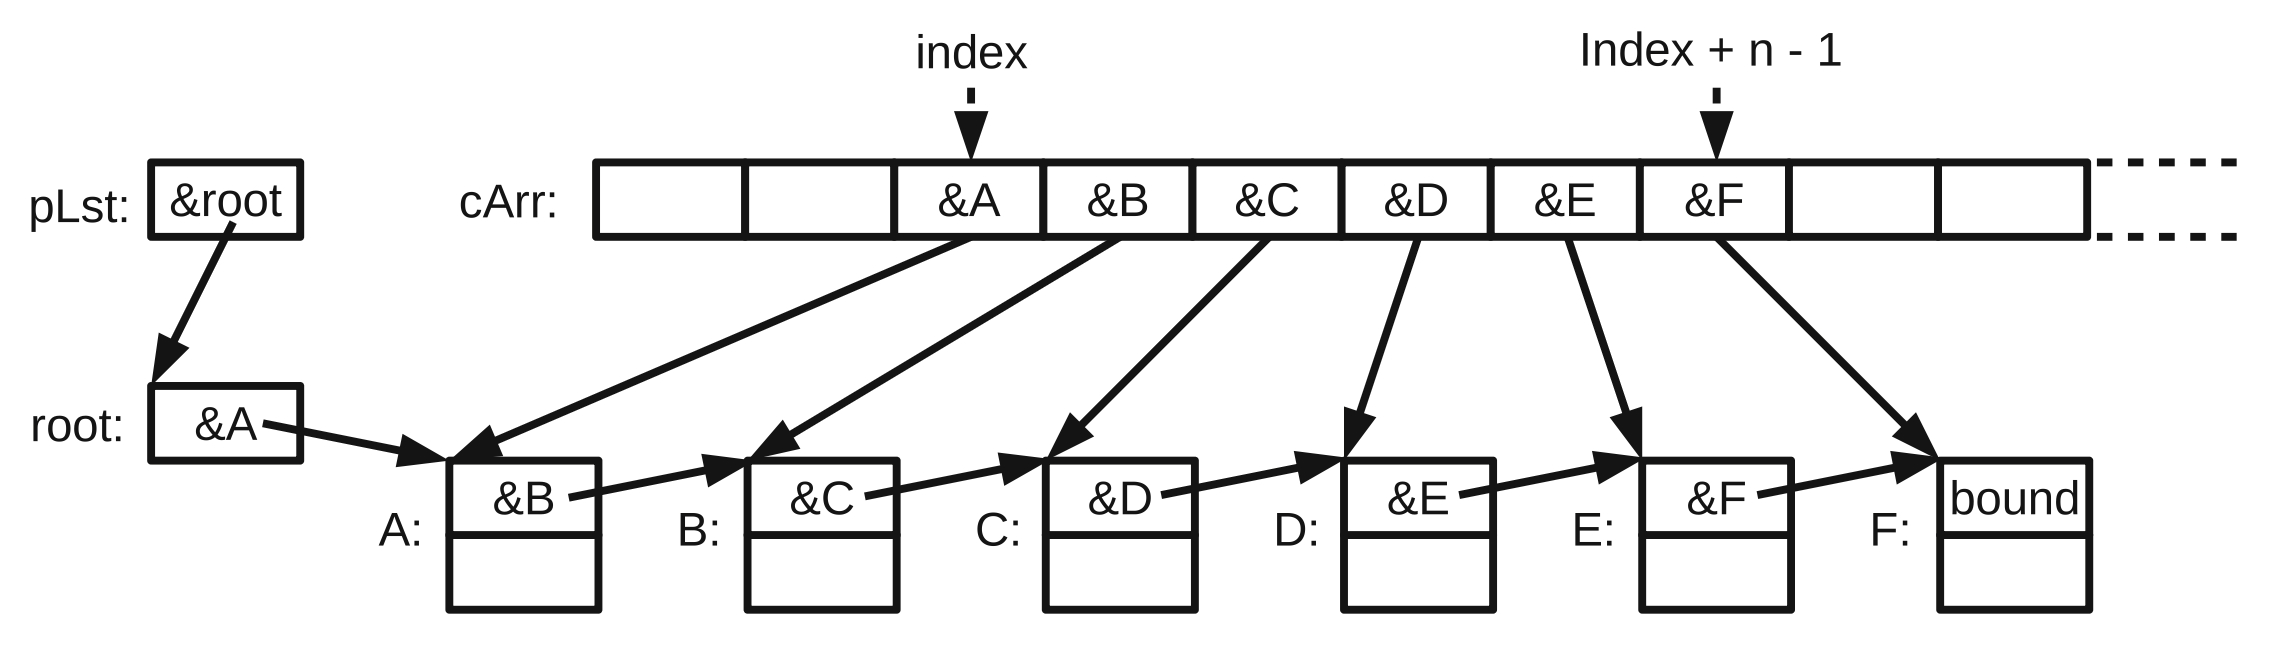
\includegraphics[width=\linewidth]{images/list-serialized}
    \caption{
        Vizualizace serializace spojového seznamu. \\
        Převzato z článku Ghosts for Lists: A Critical Module of Contiki Verified in Frama\mbox{-}C~\cite{FCGhostsForLists}.
    }
    \label{fig:linked-list-serialization}
\end{figure}

Serializace stromu, ve speciálním případě binární haldy,
lze provést pomocí mapování prvků stromu do indexů pole dle následujícího vzorce.
Pokud je prvek na indexu $i$, pak levý potomek je na indexu $2i + 1$ a pravý potomek je na indexu $2i + 2$.
Rodičovský prvek je na indexu $\lfloor \frac{i - 1}{2} \rfloor$.
V binární haldě nemůže nastat situace s prázdným nepoužitým uzlem a pole se tedy vždy plní korektně
od nejnižšího indexu po nejvyšší.
Obecné stromy by s tímto principem nemohly být serializovány,
protože je možné, že některé uzly budou prázdné a nebudou mít žádného potomka.
Řešením může být například nepoužívat jednoduchou serializaci prvků stromu do pole,
ale používat rozšířenou strukturu v serializovaném poli, která bude určovat,
zdali je daný prvek platný nebo ne.
Indexace prvků v poli by tímto přístupem byla zachována,
pouze důkazy používající tuto strukturu by musely při každém přístupu na prvek stromu
zkontrolovat, zdali je prvek platný nebo ne.
Na takto serializovaných stromech by bylo jednoduché provádět důkazy,
jelikož všechny prvky v poli jsou odděleny, a tedy splňují podmínku oddělenosti paměti.
Predikáty popisující vlastnosti stromu by musely ale obsahovat kontrolu,
zdali je daný prvek v poli platný nebo ne.

% TODO: nebo ne -> a nebo ne?

Nevýhoda serializace obecných stromů do pole je ta, že řídké stromy budou zabírat
násobně více paměti, než je potřeba.
V nejhorším případě, kdy by pomocí této metody byl zakódován strom obsahující řetězec \texttt{n} pravých uzlů,
by serializované pole reprezentující tento strom mělo velikost $2^n~-~1$ s~$2^n~-~n$ neplatnými uzly.
Další nevýhoda serializace stromových struktur spočívá v složitosti
tvořených predikátů a vlastností stromu.
Serializací ztrácíme lokální pohled na problém, který musíme nahradit prací s indexy v poli.
Lokálností rozumíme situaci, kdy je strom reprezentován ukazateli ve kterém lze snadno dokazovat vlastnosti konkrétního uzlu, jeho potomků či rodiče.
Převedením dynamické struktury do serializovaného pole se komplikuje hledání vhodného invariantu cyklu,
který se stromem v této podobě správně pracuje.

% TODO: pridat nedelitelnou mezeru tak, aby nebyly jedno-znaky na konci radku samy

%why3 config detect
%Found prover Alt-Ergo version 2.5.3, OK.
%Found prover Alt-Ergo version 2.5.3 (alternative: BV)
%Found prover Alt-Ergo version 2.5.3 (alternative: counterexamples)
%Found prover CVC4 version 1.8 (alternative: strings+counterexamples)
%Found prover CVC4 version 1.8 (alternative: strings)
%Found prover CVC4 version 1.8 (alternative: counterexamples)
%Found prover CVC4 version 1.8, OK.
%7 prover(s) added
%Save config to /home/parallels/.why3.conf


%2.3.3 Model Selection
%These options modify the underlying memory model that is used for computing weakest
%preconditions. See chapter 3 for details. Models are identified by a combination of selectors
%which are defined below:
%Selector Description
%Hoare Select Hoare memory model.
%Typed Select Typed memory model with limited casts.
%cast Select Typed memory model with unlimited casts (unsound).
%nocast Select Typed memory model with no casts.
%raw Disable the combination of memory models.
%var Combination of memory models based on variable analysis.
%ref Activate the detection of pointer variables used for reference passing style.
%caveat Caveat memory model (see 3.7).
%int Use machine integers when overflows and downcasts might occurs.
%nat Integer model without bounds (no overflow assumed).
%float Use floating-point operations.
%real Use mathematical reals instead of floating point.
